%  LaTeX support: latex@mdpi.com 
%  For support, please attach all files needed for compiling as well as the log file, and specify your operating system, LaTeX version, and LaTeX editor.

%=================================================================
\documentclass[electronics,article,submit,pdftex,moreauthors]{Definitions/mdpi} 
\usepackage{amsmath}
\usepackage{algorithm}
\usepackage{algpseudocode}
\usepackage{amssymb}
\usepackage{comment}
\usepackage{tikz}
\usepackage{subcaption}
\usetikzlibrary{shapes.geometric, arrows.meta, positioning, calc, fit}
%\documentclass[preprints,article,submit,pdftex,moreauthors]{Definitions/mdpi} 
% For posting an early version of this manuscript as a preprint, you may use "preprints" as the journal. Changing "submit" to "accept" before posting will remove line numbers.

%--------------------
% Class Options:
%--------------------
%----------
% journal
%----------
% Choose between the following MDPI journals:
% accountaudit, acoustics, actuators, addictions, adhesives, admsci, adolescents, aerobiology, aerospace, agriculture, agriengineering, agrochemicals, agronomy, ai, air, algorithms, allergies, alloys, amh, analytica, analytics, anatomia, anesthres, animals, antibiotics, antibodies, antioxidants, applbiosci, appliedchem, appliedmath, appliedphys, applmech, applmicrobiol, applnano, applsci, aquacj, architecture, arm, arthropoda, arts, asc, asi, astronomy, atmosphere, atoms, audiolres, automation, axioms, bacteria, batteries, bdcc, behavsci, beverages, biochem, bioengineering, biologics, biology, biomass, biomechanics, biomed, biomedicines, biomedinformatics, biomimetics, biomolecules, biophysica, biosensors, biosphere, biotech, birds, blockchains, bloods, blsf, brainsci, breath, buildings, businesses, cancers, carbon, cardiogenetics, catalysts, cells, ceramics, challenges, chemengineering, chemistry, chemosensors, chemproc, children, chips, cimb, civileng, cleantechnol, climate, clinbioenerg, clinpract, clockssleep, cmd, cmtr, coasts, coatings, colloids, colorants, commodities, complications, compounds, computation, computers, condensedmatter, conservation, constrmater, cosmetics, covid, crops, cryo, cryptography, crystals, csmf, ctn, curroncol, cyber, dairy, data, ddc, dentistry, dermato, dermatopathology, designs, devices, diabetology, diagnostics, dietetics, digital, disabilities, diseases, diversity, dna, drones, dynamics, earth, ebj, ecm, ecologies, econometrics, economies, education, eesp, ejihpe, electricity, electrochem, electronicmat, electronics, encyclopedia, endocrines, energies, eng, engproc, ent, entomology, entropy, environments, epidemiologia, epigenomes, esa, est, famsci, fermentation, fibers, fintech, fire, fishes, fluids, foods, forecasting, forensicsci, forests, fossstud, foundations, fractalfract, fuels, future, futureinternet, futureparasites, futurepharmacol, futurephys, futuretransp, galaxies, games, gases, gastroent, gastrointestdisord, gastronomy, gels, genealogy, genes, geographies, geohazards, geomatics, geometry, geosciences, geotechnics, geriatrics, glacies, grasses, greenhealth, gucdd, hardware, hazardousmatters, healthcare, hearts, hemato, hematolrep, heritage, higheredu, highthroughput, histories, horticulturae, hospitals, humanities, humans, hydrobiology, hydrogen, hydrology, hygiene, idr, iic, ijerph, ijfs, ijgi, ijmd, ijms, ijns, ijpb, ijt, ijtm, ijtpp, ime, immuno, informatics, information, infrastructures, inorganics, insects, instruments, inventions, iot, j, jal, jcdd, jcm, jcp, jcs, jcto, jdad, jdb, jeta, jfb, jfmk, jimaging, jintelligence, jlpea, jmahp, jmmp, jmms, jmp, jmse, jne, jnt, jof, joitmc, joma, jop, jor, journalmedia, jox, jpbi, jpm, jrfm, jsan, jtaer, jvd, jzbg, kidney, kidneydial, kinasesphosphatases, knowledge, labmed, laboratories, land, languages, laws, life, lights, limnolrev, lipidology, liquids, literature, livers, logics, logistics, lubricants, lymphatics, machines, macromol, magnetism, magnetochemistry, make, marinedrugs, materials, materproc, mathematics, mca, measurements, medicina, medicines, medsci, membranes, merits, metabolites, metals, meteorology, methane, metrics, metrology, micro, microarrays, microbiolres, microelectronics, micromachines, microorganisms, microplastics, microwave, minerals, mining, mmphys, modelling, molbank, molecules, mps, msf, mti, multimedia, muscles, nanoenergyadv, nanomanufacturing, nanomaterials, ncrna, ndt, network, neuroglia, neurolint, neurosci, nitrogen, notspecified, nursrep, nutraceuticals, nutrients, obesities, oceans, ohbm, onco, oncopathology, optics, oral, organics, organoids, osteology, oxygen, parasites, parasitologia, particles, pathogens, pathophysiology, pediatrrep, pets, pharmaceuticals, pharmaceutics, pharmacoepidemiology, pharmacy, philosophies, photochem, photonics, phycology, physchem, physics, physiologia, plants, plasma, platforms, pollutants, polymers, polysaccharides, populations, poultry, powders, preprints, proceedings, processes, prosthesis, proteomes, psf, psych, psychiatryint, psychoactives, psycholint, publications, purification, quantumrep, quaternary, qubs, radiation, reactions, realestate, receptors, recycling, regeneration, religions, remotesensing, reports, reprodmed, resources, rheumato, risks, robotics, rsee, ruminants, safety, sci, scipharm, sclerosis, seeds, sensors, separations, sexes, signals, sinusitis, siuj, skins, smartcities, sna, societies, socsci, software, soilsystems, solar, solids, spectroscj, sports, standards, stats, std, stresses, surfaces, surgeries, suschem, sustainability, symmetry, synbio, systems, tae, targets, taxonomy, technologies, telecom, test, textiles, thalassrep, therapeutics, thermo, timespace, tomography, tourismhosp, toxics, toxins, transplantology, transportation, traumacare, traumas, tropicalmed, universe, urbansci, uro, vaccines, vehicles, venereology, vetsci, vibration, virtualworlds, viruses, vision, waste, water, wem, wevj, wild, wind, women, world, youth, zoonoticdis

%---------
% article
%---------
% The default type of manuscript is "article", but can be replaced by: 
% abstract, addendum, article, benchmark, book, bookreview, briefcommunication, briefreport, casereport, changes, clinicopathologicalchallenge, comment, commentary, communication, conceptpaper, conferenceproceedings, correction, conferencereport, creative, datadescriptor, discussion, entry, expressionofconcern, extendedabstract, editorial, essay, erratum, fieldguide, hypothesis, interestingimages, letter, meetingreport, monograph, newbookreceived, obituary, opinion, proceedingpaper, projectreport, reply, retraction, review, perspective, protocol, shortnote, studyprotocol, supfile, systematicreview, technicalnote, viewpoint, guidelines, registeredreport, tutorial,  giantsinurology, urologyaroundtheworld
% supfile = supplementary materials

%----------
% submit
%----------
% The class option "submit" will be changed to "accept" by the Editorial Office when the paper is accepted. This will only make changes to the frontpage (e.g., the logo of the journal will get visible), the headings, and the copyright information. Also, line numbering will be removed. Journal info and pagination for accepted papers will also be assigned by the Editorial Office.

%------------------
% moreauthors
%------------------
% If there is only one author the class option oneauthor should be used. Otherwise use the class option moreauthors.

%---------
% pdftex
%---------
% The option pdftex is for use with pdfLaTeX. Remove "pdftex" for (1) compiling with LaTeX & dvi2pdf (if eps figures are used) or for (2) compiling with XeLaTeX.

%=================================================================
% MDPI internal commands - do not modify
\firstpage{1} 
\makeatletter 
\setcounter{page}{\@firstpage} 
\makeatother
\pubvolume{1}
\issuenum{1}
\articlenumber{0}
\pubyear{2025}
\copyrightyear{2025}
%\externaleditor{Firstname Lastname} % More than 1 editor, please add `` and '' before the last editor name
\datereceived{ } 
\daterevised{ } % Comment out if no revised date
\dateaccepted{ } 
\datepublished{ } 
%\datecorrected{} % For corrected papers: "Corrected: XXX" date in the original paper.
%\dateretracted{} % For retracted papers: "Retracted: XXX" date in the original paper.
\hreflink{https://doi.org/} % If needed use \linebreak
%\doinum{}
%\pdfoutput=1 % Uncommented for upload to arXiv.org
%\CorrStatement{yes}  % For updates
%\longauthorlist{yes} % For many authors that exceed the left citation part
%\IsAssociation{yes} % For association journals

%=================================================================
% Add packages and commands here. The following packages are loaded in our class file: fontenc, inputenc, calc, indentfirst, fancyhdr, graphicx, epstopdf, lastpage, ifthen, float, amsmath, amssymb, lineno, setspace, enumitem, mathpazo, booktabs, titlesec, etoolbox, tabto, xcolor, colortbl, soul, multirow, microtype, tikz, totcount, changepage, attrib, upgreek, array, tabularx, pbox, ragged2e, tocloft, marginnote, marginfix, enotez, amsthm, natbib, hyperref, cleveref, scrextend, url, geometry, newfloat, caption, draftwatermark, seqsplit
% cleveref: load \crefname definitions after \begin{document}

%=================================================================
% Please use the following mathematics environments: Theorem, Lemma, Corollary, Proposition, Characterization, Property, Problem, Example, ExamplesandDefinitions, Hypothesis, Remark, Definition, Notation, Assumption
%% For proofs, please use the proof environment (the amsthm package is loaded by the MDPI class).

%=================================================================
% Full title of the paper (Capitalized)
\Title{Joint UAV Trajectory Planning and LEO Satellite  Selection for Data Offloading in Space-Air-Ground  Integrated Networks}

% MDPI internal command: Title for citation in the left column
\TitleCitation{Joint UAV Trajectory Planning and LEO Satellite  Selection for Data Offloading in Space-Air-Ground  Integrated Networks}

% Author Orchid ID: enter ID or remove command
\newcommand{\orcidauthorA}{0000-0003-3080-1514} % Add \orcidA{} behind the author's name
%\newcommand{\orcidauthorB}{0000-0000-0000-000X} % Add \orcidB{} behind the author's name

% Authors, for the paper (add full first names)
\Author{Tie Liu $^{1}$\orcidA{}, Firstname Lastname $^{2}$ and Firstname Lastname $^{2,}$*}

%\longauthorlist{yes}

% MDPI internal command: Authors, for metadata in PDF
\AuthorNames{Tie Liu, Firstname Lastname and Firstname Lastname}

% Author citation:  
\AuthorCitation{L, Tie.; Lastname, F.; Lastname, F.}

% Affiliations / Addresses (Add [1] after \address if there is only one affiliation.)
\address{%
$^{1}$ \quad Affiliation 1; e-mail@e-mail.com\\
$^{2}$ \quad Affiliation 2; e-mail@e-mail.com}

% Contact information of the corresponding author
\corres{Correspondence: e-mail@e-mail.com; Tel.: (optional; include country code; if there are multiple corresponding authors, add author initials) +xx-xxxx-xxx-xxxx (F.L.)}

% Current address and/or shared authorship
%\firstnote{Current address: Affiliation.}  
% Current address should not be the same as any items in the Affiliation section.

%\secondnote{These authors contributed equally to this work.}
% The commands \thirdnote{} till \eighthnote{} are available for further notes.

%\simplesumm{} % Simple summary

%\conference{} % An extended version of a conference paper

% Abstract (Do not insert blank lines, i.e. \\) 
\abstract{The rapid development of low Earth orbit (LEO) satellites and unmanned aerial vehicles (UAVs) has positioned space–air–ground integrated networks (SAGIN) as a key architecture for next-generation IoT services. However, heterogeneous link conditions and strong temporal dynamics make reliable data collection and offloading highly challenging. This paper proposes a two-stage optimization framework for UAV-assisted IoT data acquisition and LEO satellite offloading. The first stage constructs energy-efficient UAV trajectories by jointly optimizing NOMA pairing, power allocation, and hovering locations using a hybrid gradient–combinatorial approach. The second stage introduces a Demand-Aware handover strategy that leverages mission-level sufficiency to ensure stable satellite connectivity under fast-varying orbital dynamics. Simulation results show that the proposed framework substantially reduces UAV energy consumption, shortens flight paths, and lowers handover frequency and packet loss compared with conventional methods. The two-stage design further exhibits strong scalability with respect to both IoT device density and satellite constellation size. These findings demonstrate the effectiveness of modular yet complementary optimization across heterogeneous SAGIN segments and provide actionable guidelines for the deployment of integrated aerial–satellite IoT systems.}

% Keywords
\keyword{SAGIN, UAV communications, satellite networks, mixed-integer optimization, trajectory design, mobility management.} 

% The fields PACS, MSC, and JEL may be left empty or commented out if not applicable
%\PACS{J0101}
%\MSC{}
%\JEL{}

%%%%%%%%%%%%%%%%%%%%%%%%%%%%%%%%%%%%%%%%%%
% Only for the journal Diversity
%\LSID{\url{http://}}

%%%%%%%%%%%%%%%%%%%%%%%%%%%%%%%%%%%%%%%%%%
% Only for the journal Applied Sciences
%\featuredapplication{Authors are encouraged to provide a concise description of the specific application or a potential application of the work. This section is not mandatory.}
%%%%%%%%%%%%%%%%%%%%%%%%%%%%%%%%%%%%%%%%%%

%%%%%%%%%%%%%%%%%%%%%%%%%%%%%%%%%%%%%%%%%%
% Only for the journal Data
%\dataset{DOI number or link to the deposited data set if the data set is published separately. If the data set shall be published as a supplement to this paper, this field will be filled by the journal editors. In this case, please submit the data set as a supplement.}
%\datasetlicense{License under which the data set is made available (CC0, CC-BY, CC-BY-SA, CC-BY-NC, etc.)}

%%%%%%%%%%%%%%%%%%%%%%%%%%%%%%%%%%%%%%%%%%
% Only for the journal BioTech, Fishes, Neuroimaging and Toxins
%\keycontribution{The breakthroughs or highlights of the manuscript. Authors can write one or two sentences to describe the most important part of the paper.}

%%%%%%%%%%%%%%%%%%%%%%%%%%%%%%%%%%%%%%%%%%
% Only for the journal Encyclopedia
%\encyclopediadef{For entry manuscripts only: please provide a brief overview of the entry title instead of an abstract.}

%%%%%%%%%%%%%%%%%%%%%%%%%%%%%%%%%%%%%%%%%%
% Different journals have different requirements. Please check the specific journal guidelines in the "Instructions for Authors" on the journal's official website.
%\addhighlights{yes}
%\renewcommand{\addhighlights}{%
%
%\noindent The goal is to increase the discoverability and readability of the article via search engines and other scholars. Highlights should not be a copy of the abstract, but a simple text allowing the reader to quickly and simplified find out what the article is about and what can be cited from it. Each of these parts should be devoted up to 2~bullet points.\vspace{3pt}\\
%\textbf{What are the main findings?}
% \begin{itemize}[labelsep=2.5mm,topsep=-3pt]
% \item First bullet.
% \item Second bullet.
% \end{itemize}\vspace{3pt}
%\textbf{What is the implication of the main finding?}
% \begin{itemize}[labelsep=2.5mm,topsep=-3pt]
% \item First bullet.
% \item Second bullet.
% \end{itemize}
%}

%%%%%%%%%%%%%%%%%%%%%%%%%%%%%%%%%%%%%%%%%%
\begin{document}

%%%%%%%%%%%%%%%%%%%%%%%%%%%%%%%%%%%%%%%%%%
%\endnote{This is an endnote.} % To use endnotes, please un-comment \printendnotes below (before References). Only journal Laws uses \footnote.

% The order of the section titles is different for some journals. Please refer to the "Instructions for Authors” on the journal homepage.

\section{Introduction}

The Internet of Things (IoT) devices are widely applied in the daily life, such as environmental monitoring and traffic management. However, due to the limited ground base stations in remote or post-disaster areas, it is difficult to satisfy the demands for data collection and offloading supported by the terrestrial networks. The space-air-ground integrated network (SAGIN) is perceived as an effective solution to tackle the above difficulties \cite{jia2020leo}.In SAGIN, low earth orbit (LEO) satellites can provide the IoT devices with extensive connectivities \cite{xiao2024space} \cite{duan2022distributed}.Additionally, the in-orbit computing allows LEO satellites to directly process tasks, which avoids the long propagation delays and eases the congestion on bandwidthlimited downlink channels\cite{wei2024energy} \cite{pan2022latency}.Moreover, unmanned aerial vehicles (UAVs), as ideal candidates for aerial relays, can be deployed flexibly to ensure efficient data collection \cite{jia2025distributionally}.On one hand, the UAVs trajectories can be optimized to minimize the multi-hop transmission and propagation distance \cite{mao2020joint}.Besides, UAVs facilitate the line-of-sight (LoS) communications with ground devices for a wide view, improving the channel quality and enhancing the transmission throughput  \cite{zhao2021multi} \cite{mozaffari2019tutorial}.Nevertheless, the limitation of communication resources restricts the number of IoT devices served by UAVs and leads to a poor spectrum efficiency \cite{tao2015survey}.In response to this issue, the non-orthogonal multiple access (NOMA) technology, which emerges as a promising paradigm, allows multiple IoT devices to share a single resource block.

Some works have begun to explore problems on resource allocations in SAGIN.The authors in \cite{fang2022noma} propose an iterative power allocation algorithm to maximize the sum rate in a NOMA-based hybrid satellite-UAV-terrestrial network.In \cite{jia2025service}, the authors consider the complexity of SAGIN and sovle the service function chain scheduling problem by incorporating deep reinforcement learning.The authors in \cite{huang2024joint} study the total energy consumption minimization for task processing in an SAGIN-supported mobile edge computing system.In \cite{jia2024dynamic}, the authors introduce a data collection scheme to balance the throughput and fairness among the IoT nodes in SAGIN. Although the above works are conducted in SAGIN, the satellite selection issues are not considered, which can significantly enhance the performance of the system.

Given the instability and time-varying nature of heterogeneous communications within the SAGIN system, we propose a hierarchical framework integrating ground-based IoT devices, unmanned aerial vehicles (UAVs) serving as aerial relays, and computationally capable low-Earth orbit satellites. The problem is modelled as minimising total UAV energy consumption whilst ensuring service quality guarantees. To address this, the process is divided into two phases. In Phase One, we design algorithms for IoT pairing, power allocation, and UAV trajectory planning. In the second phase, we introduce a demand-aware flexible switching mechanism for low-Earth orbit satellites.

The remainder of this paper is organized as follows. In Section II, we design the system model and provide the problem formulation. In Section III, the algorithms are proposed. Section IV evaluates the performance of the proposed algorithms via numerical analyses. Finally, the conclusions are drawn in Section V.
%%%%%%%%%%%%%%%%%%%%%%%%%%%%%%%%%%%%%%%%%%
\section{Materials and Methods}

As shown in Figure~\ref{fig:system_model}, we consider an SAGIN which consists of $\mathbf{U}$ UAVs denoted by $\mathcal{U} = \{1, 2, \dots, U\}$, and $\mathbf{S}$ LEO satellites indicated by  $\mathcal{S} = \{1, 2, \dots, S\}$. In addition, $\mathbf{K}$ IoT devices scattered randomly on the ground are represented as $\mathcal{K} = \{1, 2, \dots, K\}$.Due to the limited computational capabilities of IoT terminals, the data they collect must be uploaded to low-Earth orbit satellites for further processing. However, constrained by their own energy and transmission power limitations, IoT devices struggle to communicate directly with these satellites. To address this, we introduce drones as aerial base stations to assist in data aggregation and forwarding within target areas. Based on this architecture, the data upload process can be divided into two stages. In the first stage, the UAV follows a pre-planned flight path to sequentially reach multiple hovering positions, collecting data generated by IoT devices within the area before returning to the starting point upon completion. In the second stage, after returning to the starting point, the UAV hovers at the origin and selects an appropriate LEO satellite to perform computational offloading tasks.
% Figure 1
\begin{figure}[!htbp]
\centering
\includegraphics[width=0.95\columnwidth]{Definitions/figure1}
\caption{System model of the Space-Air-Ground Integrated Network (SAGIN) showing IoT devices, UAVs, and LEO satellites.}
\label{fig:system_model}
\end{figure}
\subsection{Data Collection from IoT to UAV}

During the data upload phase for IoT devices and drones, we introduce Non-Orthogonal Multiple Access (NOMA) technology to enhance the system's spectrum efficiency and transmission effectiveness. Specifically, we assume that within a defined spatial range, any two IoT devices can form a cooperative pair, transmitting their uplink data simultaneously to the UAV via the NOMA mechanism. For devices that cannot meet pairing conditions or fail to pair successfully, Orthogonal Frequency Division Multiple Access (OFDMA) is employed for independent data transmission.
% Figure  2
\begin{figure}[!htbp]
\centering
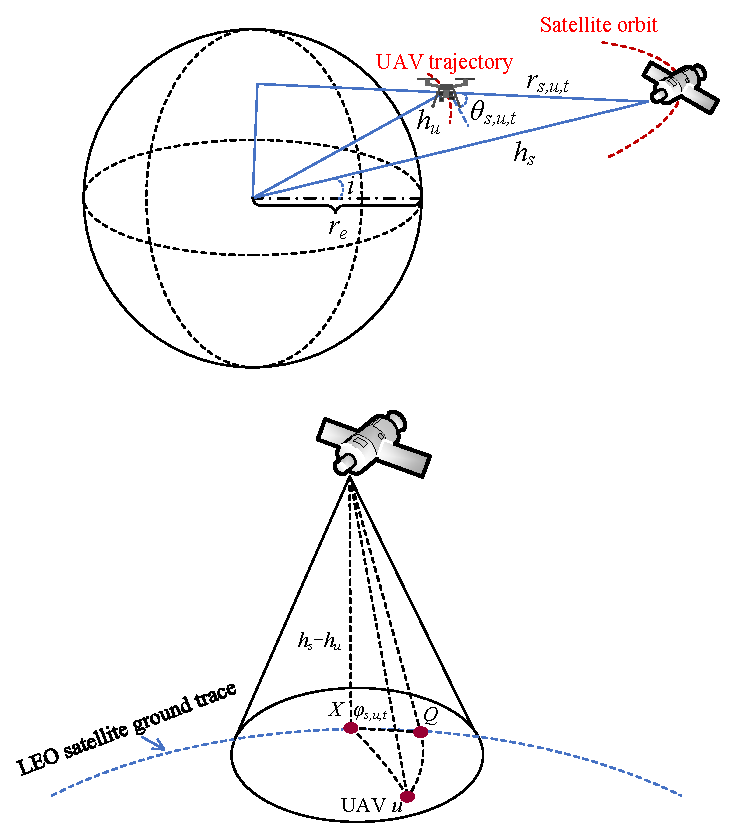
\includegraphics[width=0.95\columnwidth]{Definitions/figure2}
\caption{Geometrical representation of UAV-LEO communication link parameters.}
\label{fig:uav_leo_geometry}
\end{figure}

A three-dimensional Cartesian coordinate system is employed to characterize the spatial locations of UAVs and IoT devices. The IoT devices are assumed to be randomly distributed on the ground plane, and the horizontal coordinate of the $k$-th device denoted as $\mathbf{q}_k = (x_k, y_k, 0)$. Each UAV operates at a fixed altitude $h_u$. Accordingly, the position of the $u$-th UAV at the $n$-th hover point is expressed as $\mathbf{q}_u(n) = (x_u(n), y_u(n), h_u)$. Due to the elevated UAV altitude and the unobstructed propagation environment, the wireless links between IoT devices and UAVs are dominated by line-of-sight (LoS) propagation. Under this condition, the channel gain between IoT device $k$ and its associated UAV is modeled as
\begin{quote}
\begin{equation}
G_k = \frac{\beta_0}{h_u^2 + (x_u(n) - x_k)^2 + (y_u(n) - y_k)^2},
\end{equation}
\end{quote}
where $\beta_0$ represents the channel gain at the reference distance $r_0$ = 1m.

Let $\mathcal{P}$ denote the set of all feasible transmission pairs, where each pair $p \in \mathcal{P}$ consists of either (i) two IoT devices forming a NOMA cluster or (ii) a single device operating in OFDMA mode. A binary decision variable $\delta_{p} \in \{0,1\}$ is introduced to indicate whether pair $p$ is activated. To ensure that each IoT device is assigned to at most one pair, the following constraint is imposed
\begin{quote}
\begin{equation}
\sum_{p \in P: k \in p} \delta_p \leq 1, \quad \forall k \in \mathcal{K}.
\end{equation}
\end{quote}

For an activated NOMA pair containing two devices $p = \{k, m\}$, the device with the stronger channel gain performs successive interference cancellation (SIC) and decodes the weaker device’s signal prior to decoding its own signal. The corresponding interference structure is determined by the activated pair $p$.

Given the pairing configuration, the received signal-to-interference-plus-noise ratio (SINR) of IoT device $k$ can be expressed as
\begin{quote}
\begin{equation}
\mathrm{SINR}_k = \frac{p_k G_k}{\sum_{\substack{p \in P \\ k,m \in p \\ m \neq k}} \delta_p p_m G_m + \sigma_{iu}^2},
\end{equation}
\end{quote}
where $p_k$ s the transmit power of device $k$, and $\sigma^2 _{iu}$ denotes the receiver noise power. Based on the obtained SINR, the achievable uplink data rate of device $k$ is
\begin{quote}
\begin{equation}
d_k = B_{iu} \log_2 \left(1 + \mathrm{SINR}_k\right),
\end{equation}
\end{quote}
where $B_{iu}$ represents the bandwidth allocated to UAV–IoT communications. Given the task data size $D_k$, the corresponding uplink transmission delay is
\begin{quote}
\begin{equation}
T_k^{{tr}} = \frac{D_k}{d_k},
\end{equation}
\end{quote}

A predetermined visiting order is assumed for each UAV to sequentially approach all NOMA groups and independent IoT devices after its trajectory has been determined. The trajectory of UAV $u$ is represented by the ordered set $\{\mathbf{q}_u(0), \mathbf{q}_u(1), \dots, \mathbf{q}_u(N_u)\}$, where $N_u$ denotes the number of hovering waypoints assigned to UAV $u$. Accordingly, the total flight path length of UAV $u$ over the entire mission is defined as
\begin{equation}
L_u = \sum_{n=0}^{N_u-1} \lVert \mathbf{q}_u(n+1) - \mathbf{q}_u(n) \rVert.
\end{equation}

Given a constant flight speed $v_f$, the required flight time for UAV $u$ is expressed as
\begin{equation}
T^{fly}_u = \frac{L_u}{v_f}.
\end{equation}

During the data collection phase, each UAV hovers at designated waypoints to receive data from IoT devices. The hovering duration of UAV $u$ is determined by the transmission times of all devices within the active pairs. Based on the pair-based NOMA definition, the hovering time is expressed as
\begin{equation}
T_u^{hov} = \sum_{p \in P} \delta_p \max_{k \in p} \frac{D_k}{d_k}.
\end{equation}

For NOMA pairs containing two devices, the maximum operator ensures that UAV $u$ hovers sufficiently long to receive the data from both devices in parallel, whereas for single-device OFDMA pairs, the expression reduces to the corresponding device’s transmission time.

The energy consumption of UAV $u$ in this phase comprises both hovering energy and flight-related energy. Accordingly, the total energy consumption of the UAV–IoT subsystem is
\begin{equation}
E_{total} = \sum_{u=1}^{U} (P_h T_u^{hov} + P_f T_u^{fly}),
\end{equation}
where $P_h$ and $P_f$ represent the hovering power and flight power of the UAVs, respectively, and $T^{fly}_u$ is the flight time of UAV $u$ as defined previously.

\subsection{Data Offloading from UAV to LEO}

After the UAV completes data collection from all IoT devices, it acquires the position information of all visible LEO satellites and selects the satellite that can satisfy the transmission demand. To represent the computation offloading decision, a binary association variable $\beta_{s,u,t} \in \{0, 1\}$ is introduced, where $\beta_{s,u,t} = 1$ indicates that UAV $u$ offloads its computation to satellite $s$ at time $t$. The channel gain between UAV $u$ and LEO satellite $s$ is modeled based on the free-space path loss as
\begin{equation}
G_{s,u,t}[dB] = 92.44 + 20\log_{10}(r_{s,u,t}) +20\log_{10}(f_s),
\end{equation}
where $f_s$ denotes the operating frequency of satellite $s$ in GHz, and $r_{s,u,t}$ is the straight-line distance between UAV $u$ and satellite $s$ at $t$. The distance $r_{s,u,t}$ is calculated according to the geometry of the Earth–UAV–satellite system
\begin{equation}
r_{s,u,t} = \sqrt{(r_e + h_s)^2 + (r_e + h_u)^2 - 2(r_e + h_s)(r_e + h_u) \cos \theta_{s,u,t}},
\end{equation}
where $r_e$ is the Earth radius, and $h_u$ and $h_s$ are the altitudes of the UAV and LEO satellite, respectively. The satellite elevation angle $\theta_{s,u,t}$ with respect to UAV $u$ according to \cite{seyedi2012trace} is computed as
\begin{equation}
\theta_{s,u,t} = \arctan \left( \frac{h_s - h_u}{d_{\mathrm{ground},s,u,t}} \right), \quad d_{\mathrm{ground},s,u,t} = r_e \phi_{s,u,t},
\end{equation}
where $d_{\mathrm{ground},s,u,t}$ is the horizontal distance on the Earth surface between UAV $u$ and the sub-satellite point of satellite $s$, and $\phi_{s,u,t}$ denotes the corresponding central angle on the Earth’s surface. The central angle $\phi_{s,u,t}$ varies over time according to the satellite and Earth motion
\begin{equation}
\phi_{s,u,t} = (\omega_E \cos i - \omega_S)(t - t_0) + \phi_{s,u,t_0},
\end{equation}
where $\omega_E$,  $\omega_S$ are the angular velocities of the Earth rotation and satellite orbit, $i$ is the orbital inclination of the satellite, $t_0$ is the time when the satellite becomes visible to the UAV, and $\phi_{s,u,t_0}$ is the initial central angle at $t_0$.

The received power at LEO satellite $s$ from UAV $u$ at time $t$ is expressed as
\begin{equation}
P_{s,u,t}^{re} = P_{tr} G_{tr} G_{re} G_{s,u,t}^{lin},
\end{equation}
where $P_{tr}$ denotes the transmit power of the UAV, $G_{tr}$ and $G_{re}$ are the transmit and receive antenna gains of the UAV and LEO satellite, respectively, and $G_{s,u,t}^{lin}$ is the linear-scale channel gain between UAV $u$ and satellite $s$, derived from the distance-dependent free-space path loss as described in subsection 2.1.

Based on the received power, the achievable uplink data rate from UAV $u$ to LEO satellite $s$ at time $t$ is calculated according to the Shannon capacity formula
\begin{equation}
d_{s,u,t} = B_{su} \log_2 \left(1 + \frac{P_{s,u,t}^{re}}{\sigma_{su}^2}\right),
\end{equation}
where $B_{su}$ denotes the available bandwidth of the UAV–LEO link, and $\sigma_{su}^2$ is the noise power at the satellite receiver. Let $x_{s,u,t} \in \{0,1\}$ represent the satellite association decision, where $x_{s,u,t} = 1$ indicates that UAV $u$ connects to satellite $s$ at time $t$.To characterize unnecessary switching, the handover indicator is defined as
\begin{equation}
 h_{u,t} = \frac{1}{2} \sum_{s=1}^{S} |x_{s,u,t} - x_{s,u,t-1}|.
\end{equation}

\subsection{Problem Formulation}

To minimize the total energy consumption of the first-stage IoT–UAV data collection process, the optimization is performed over the pair-based association variables $\boldsymbol{\delta} = \{\delta_p \mid p \in P\}$, the transmit power allocation of IoT devices $\mathbf{p} = \{p_k \mid k \in K\}$, and the UAV hovering positions and visiting order $\mathbf{q} = \{\mathbf{q}_u(n) \mid u \in U\}$. By jointly optimizing $\boldsymbol{\delta}$, $\mathbf{p}$, and $\mathbf{q}$, , the total UAV energy consumption consisting of hovering and flight energy is minimized. The optimization problem is detailed as
\begin{subequations}
\begin{align}
\mathcal{P}_1: \min_{\delta, \mathbf{p}, \mathbf{q}} \quad & 
\sum_{u=1}^{U} \left( P_h \sum_{p \in P_u} \delta_p \max_{k \in p} \frac{D_k}{d_k} + P_f \frac{L_u}{v_f} \right) \\
\text{s.t.} \quad & p_{\min} \leq p_k \leq p_{\max}, \quad \forall k, \label{eq:p1_power} \\
& \sum_{p: k \in p} \delta_p \leq 1, \quad \forall k, \label{eq:p1_assignment} \\
& \rho p_{i(p)} G_{i(p)} \leq p_{j(p)} G_{j(p)}, \quad \forall p \in P_{\text{NOMA}}, \label{eq:p1_noma} \\
& \mathbf{q}_u(N_u) = \mathbf{q}_u(0), \quad \forall u, \label{eq:p1_trajectory} \\
& \delta_p \in \{0, 1\}, \quad \forall p \in P. \label{eq:p1_binary}
\end{align}
\end{subequations}

Constraint \ref{eq:p1_power} restricts the transmit power of each IoT device within its allowable operating range. Constraint  \ref{eq:p1_assignment} ensures that each device can participate in at most one transmission group, thereby preventing conflicting pair assignments. Constraint \ref{eq:p1_noma} enforces the power-domain separation required for successful NOMA decoding in every selected NOMA pair, where $\rho \in (0,1)$ denotes the minimum ratio ensuring the correct decoding order. Constraint \ref{eq:p1_trajectory} guarantees that each UAV completes a closed trajectory, returning to its initial hovering point after visiting all designated positions. Constraint \ref{eq:p1_binary} defines the binary nature of the group-selection variables.

Due to the coupling among the discrete pairing decisions $\delta_p$, the continuous transmit-power variables $\{p_k\}$, and the UAV trajectory variables $\mathbf{q}_u(n)$, the overall optimization problem P1 forms a mixed-integer nonlinear programming model, which is NP-hard and computationally intractable to solve optimally.

After completing the IoT data-collection stage, the UAV proceeds to offload its aggregated task data to LEO satellites. The primary objective of the second-stage satellite association problem is to minimize unnecessary handover frequency while meeting operational offloading requirements, thereby enhancing QoS assurance and indirectly reducing both transmission energy consumption and handover energy consumption for unmanned aerial vehicles.

Demand-Aware  Handover does not seek to solve an optimal global objective function, but rather proposes a strategy algorithm that satisfies the following constraints
\begin{subequations}
\begin{align}
\mathcal{P}_2: \min \quad & 
\sum_{u=1}^{U} \sum_{t=1}^{T} h_{u,t} \\
\text{s.t.} \quad & \sum_{s=1}^{S} \sum_{t=1}^{T} x_{s,u,t} d_{s,u,t} \Delta t \geq D_u, \quad \label{eq:p2_total}\\
&\sum_{s=1}^{S} x_{s,u,t} \leq 1, \quad \forall t \in \mathcal{T}, \label{eq:p2_visible} \\
& \theta_{s,u,t} \geq \theta_{\min}, \quad \label{eq:p2_elevation} \\
& \sum_{s=1}^{S} \sum_{t'=t}^{T} x_{s,u,t'} d_{s,u,t'} \Delta t \geq D_u^{rem}(t). \label{eq:p2_remaining} 
\end{align}
\end{subequations}

Constraint \ref{eq:p2_total} represents the total amount of data successfully offloaded during the mission must satisfy $D_u$ is the task data size to be transmitted. Constraint \ref{eq:p2_visible} represents communication continuity requires that the UAV is associated with at most one visible satellite at any time. Constraint \ref{eq:p2_elevation} represents only satellites satisfying the minimum elevation constraint are eligible for association. Constraint \ref{eq:p2_remaining} ensures that switching is triggered only when the current satellite can no longer satisfy the remaining demand under predicted link evolution where $D_u^{rem}(t)$ denotes the remaining data to be uploaded at time $t$.

\section{ALGORITHM DESIGN}

The model is divided into two stages to achieve an effective solution. Specifically: during the data transmission phase from IoT devices to drones, Algorithm 1 completes IoT pairing, power allocation, and drone flight path planning; during the data transmission phase from drones to low-orbit satellites, Algorithm 2 selects link-demand-aware low-orbit satellites to ensure QoS.

\subsection{UAV Data Collection and Energy Optimization}

To effectively solve problem $\mathcal{P}_1$, the total energy consumption in the IoT-UAV phase is considered. Since the IoT transmission energy is negligible compared to UAV hovering and flight energy, the optimization focuses on minimizing the UAV energy consumption, which consists of hovering energy and flight energy. The problem involves coupled discrete pairing decisions $\delta = \{\delta_p | p \in \mathcal{P}\}$, continuous transmit power variables $\mathbf{p} = \{p_k | k \in \mathcal{K}\}$, and UAV hovering positions $\mathbf{q} = \{\mathbf{q}_u(n) | u \in \mathcal{U}\}$. This mixed-integer nonlinear programming problem is challenging to solve directly. Therefore, an algorithm framework based on alternating optimization and local search is proposed, as illustrated in Figure~\ref{fig:algorithm_flowchart} and detailed in Algorithm~1.

The initial NOMA pairs are constructed based on distance constraints. Specifically, the distance matrix among all IoT devices is computed, and NOMA pairs are formed by grouping the two nearest devices that satisfy the pairing constraint into the pair set $\mathcal{P}$. This process repeats until no new valid pairs can be formed, and the remaining devices operate as independent OFDMA nodes.

For each activated pair $p \in \mathcal{P}$ with $\delta_p = 1$, an alternating optimization strategy is adopted to jointly optimize power allocation and hovering positions. Given fixed UAV hovering position $(x_u, y_u, h_u)$, the transmit powers of paired devices are iteratively updated using Newton's method. For a NOMA pair $p = \{k, m\}$, $p_m$ is alternately updated while fixing $p_k$ and vice versa until convergence. For independent OFDMA nodes, $p_k = p_{\max}$ is directly set to maximize throughput.

Given fixed power allocation, the UAV hovering position $(x_u, y_u)$ (with altitude $h_u$ kept fixed) is optimized using the Adam optimizer. Unlike gradient-free methods, Adam leverages adaptive learning rates and momentum to achieve faster convergence and finer position adjustments. The position update rule is given by:
\begin{align}
\mathbf{m}_t &= \beta_1 \mathbf{m}_{t-1} + (1-\beta_1)\nabla_{\mathbf{q}} E_{\text{total}}, \\
\mathbf{v}_t &= \beta_2 \mathbf{v}_{t-1} + (1-\beta_2)(\nabla_{\mathbf{q}} E_{\text{total}})^2, \\
\mathbf{q}_u^{(t+1)} &= \mathbf{q}_u^{(t)} - \alpha \frac{\hat{\mathbf{m}}_t}{\sqrt{\hat{\mathbf{v}}_t} + \epsilon},
\end{align}
where $\mathbf{m}_t$ and $\mathbf{v}_t$ are the first and second moment estimates, $\alpha$ is the learning rate, and $\beta_1, \beta_2$ are decay rates. The alternating optimization process iterates until reaching the maximum iteration count $J$ or until the objective function change falls below a threshold.

After obtaining all hovering positions, the UAV visiting order must be planned to minimize flight distance. This problem is essentially a variant of the multiple traveling salesman problem (mTSP). The 2-opt local search algorithm is employed for trajectory optimization. The 2-opt algorithm iteratively removes two edges from the trajectory and reconnects them to eliminate path crossings, thereby progressively improving solution quality until reaching a local optimum. Compared to metaheuristic methods, 2-opt provides faster convergence and more stable performance for trajectory optimization.

To further reduce energy consumption, a pair recombination mechanism is introduced. All unpaired nodes are traversed to check if there exist opportunities to recombine with existing paired nodes. If an unpaired node is closer to one member of an existing pair, the original pair is broken and a new NOMA pair is formed. For two spatially close NOMA pairs, their members are exchanged to reduce UAV flight distance or hovering time.

After each recombination or exchange operation, the UAV trajectory and total energy consumption are recalculated. The new configuration is accepted if it yields lower energy consumption; otherwise, the original configuration is retained. Through multiple rounds of exchange operations, the algorithm can escape local optima and obtain better NOMA pairing schemes. The complete algorithm flow is presented in Algorithm~1 with the corresponding flowchart shown in Figure~\ref{fig:algorithm_flowchart}.

\begin{figure*}[!t]
\centering
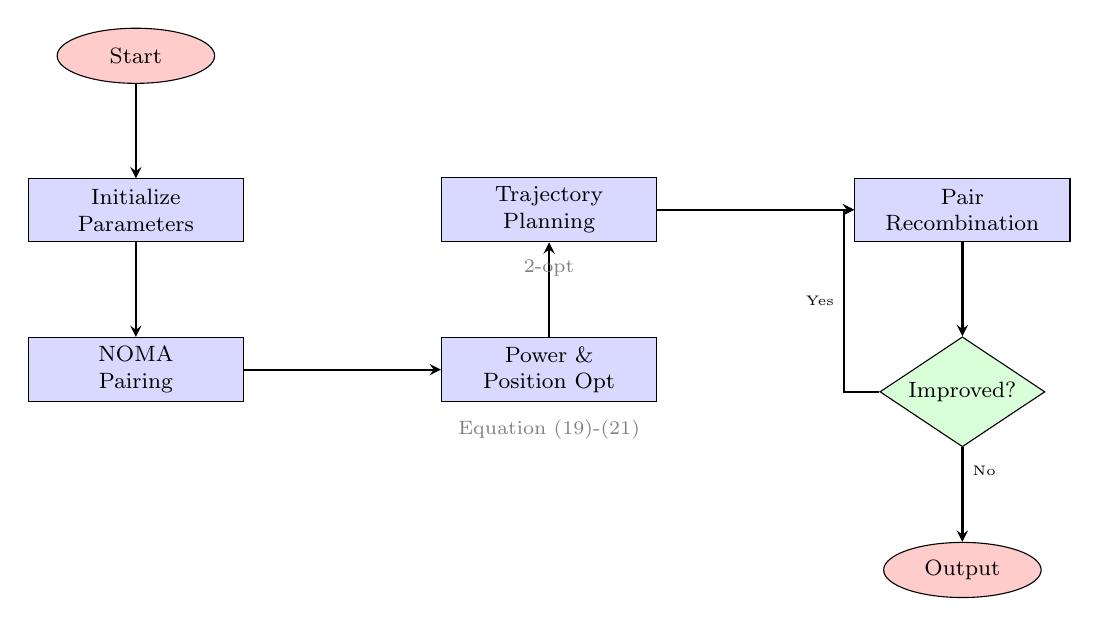
\begin{tikzpicture}[
    node distance=1.2cm and 2.5cm,
    startstop/.style={ellipse, draw, fill=red!20, text centered, minimum height=0.7cm, minimum width=2cm, font=\footnotesize},
    process/.style={rectangle, draw, fill=blue!15, text centered, text width=2.5cm, minimum height=0.8cm, font=\footnotesize},
    decision/.style={diamond, draw, fill=green!15, text centered, minimum height=1cm, minimum width=1cm, aspect=1.5, font=\footnotesize, inner sep=2pt},
    arrow/.style={thick,->,>=stealth}
]

% 第一列(从上到下)
\node (start) [startstop] {Start};
\node (init) [process, below=of start] {Initialize\\Parameters};
\node (pairing) [process, below=of init] {NOMA\\Pairing};

% 第二列(从下到上)
\node (optimization) [process, right=of pairing] {Power \&\\Position Opt};
\node (trajectory) [process, above=of optimization] {Trajectory\\Planning};

% 第三列(从上到下)
\node (exchange) [process, right=of trajectory] {Pair\\Recombination};
\node (check) [decision, below=of exchange] {Improved?};
\node (stop) [startstop, below=of check] {Output};

% 主流程箭头
\draw [arrow] (start) -- (init);
\draw [arrow] (init) -- (pairing);
\draw [arrow] (pairing) -- node[midway, below, font=\tiny] {} (optimization);
\draw [arrow] (optimization) -- (trajectory);
\draw [arrow] (trajectory) -- node[midway, below, font=\tiny] {} (exchange);
\draw [arrow] (exchange) -- (check);
\draw [arrow] (check) -- node[near start, right, font=\tiny] {No} (stop);

% 反馈循环:从check向左转弯再向上到exchange
\draw [arrow] (check) -- ++(-1.5,0) |- node[near start, left, font=\tiny] {Yes} (exchange);

% 可选:添加小注释框(使用虚线边框,放在节点下方)
\node[below=0.1cm of optimization, font=\scriptsize, text=gray] {Equation (19)-(21)};
\node[below=0.1cm of trajectory, font=\scriptsize, text=gray] {2-opt};

\end{tikzpicture}
\caption{Flowchart of the proposed algorithm for UAV data collection and energy optimization.}
\label{fig:algorithm_flowchart}
\end{figure*}

\begin{algorithm}[!htbp]
\caption{UAV Data Collection and Energy Optimization}
\label{alg:p1_optimization}
\begin{algorithmic}[1]
\State \textbf{Input:} All IoT devices' positions $\mathbf{q}_k$ and corresponding packets $D_k$, UAV initial position $\mathbf{q}_u(0)$
\State \textbf{Output:} Energy consumption $E_{\text{total}}$
\State Initialize distance matrix and maximum iterations $J$
\State Form NOMA pairs from two nearest devices under distance constraints
\State Obtain lists of paired and unpaired nodes
\For{each paired nodes $(k, m)$}
    \State Initialize transmission powers $p_k, p_m$
    \State Initialize hover position $(x_u, y_u, h_u)$
    \State Set iteration counter $j \leftarrow 0$
    \While{$j \leq J$}
        \State Update $p_k^{(j)}, p_m^{(j)}$ using Newton's method
        \State Update $(x_u^{(j)}, y_u^{(j)}, h_u)$ using Adam optimizer
        \State $j \leftarrow j + 1$
    \EndWhile
\EndFor
\State Optimize UAV trajectories using 2-opt local search
\State Compute energy consumption $E_{\text{total}}$ using Equation~(9)
\For{each node combination (unpaired and paired)}
    \State Exchange nodes between paired and unpaired groups
    \State Update UAV trajectories and device transmission powers
    \State Calculate new energy consumption $E_{\text{new}}$ using Equation~(9)
    \If{$E_{\text{new}} < E_{\text{total}}$}
        \State $E_{\text{total}} \leftarrow E_{\text{new}}$
    \EndIf
\EndFor
\State \Return $E_{\text{total}}$
\end{algorithmic}
\end{algorithm}

\subsection{LEO Satellite Selection Optimization}

After the UAV completes data collection from all IoT devices, it must offload the aggregated data to LEO satellites for further processing. Unlike static ground stations, LEO satellites exhibit high mobility with time-varying channel conditions and limited visibility windows. Consequently, the satellite association decision directly impacts both transmission efficiency and handover frequency.Frequent satellite handovers introduce signaling overhead, packet loss, and interruption delays, degrading quality of service. Conversely, maintaining connection with a suboptimal satellite prolongs transmission time and increases energy consumption. Therefore, the selection strategy must balance handover frequency against link quality to ensure timely and reliable data offloading.

To address problem P2, a demand-aware satellite selection mechanism is proposed. Rather than myopically selecting the satellite with maximum instantaneous throughput at each time slot, the algorithm evaluates whether the current satellite can satisfy the remaining data transmission demand under predicted link evolution. Satellite handover is triggered only when the current satellite is predicted to be insufficient for completing the remaining task, thereby minimizing unnecessary switching while ensuring transmission deadlines.


The algorithm operates as follows. At each decision epoch, all LEO satellites satisfying the elevation angle constraint $\theta_{s,u,t} \geq \theta_{\min}$ are identified as candidate satellites. For each candidate $s$, the instantaneous uplink data rate $d_{s,u,t}$ is calculated according to Equation (15) based on the distance-dependent channel gain and transmit power. The algorithm then predicts the cumulative throughput achievable by the current satellite over the remaining visibility window. If the predicted throughput exceeds the remaining data size $D_u^{\text{rem}}(t)$, the current satellite association is maintained. Otherwise, the algorithm selects the satellite with maximum instantaneous throughput from the candidate set and performs handover.

\begin{algorithm}[!htbp]
\caption{Demand-Aware LEO Satellite Selection}
\label{alg:satellite_selection}
\begin{algorithmic}[1]
\State \textbf{Input:} UAV position $\mathbf{q}_u(t)$, total data size $D_u$, transmitted data $D_u^{\text{tx}}$, current satellite $s_{\text{curr}}$, time $t$, prediction horizon $\Delta t$
\State \textbf{Output:} Selected satellite $s^*$
\State Compute remaining data: $D_u^{\text{rem}}(t) \gets D_u - D_u^{\text{tx}}$
\State Initialize candidate set: $\mathcal{S}_{\text{candidate}} \gets \emptyset$
\For{each satellite $s \in \mathcal{S}$}
    \State Compute elevation angle $\theta_{s,u,t}$ using Equation~(12)
    \If{$\theta_{s,u,t} \geq \theta_{\min}$}
        \State Add $s$ to $\mathcal{S}_{\text{candidate}}$
    \EndIf
\EndFor
\If{$s_{\text{curr}} \in \mathcal{S}_{\text{candidate}}$}
    \State Compute current throughput: $d_{s_{\text{curr}},u,t}$ using Equation~(15)
    \State Predict remaining visibility time: $T_{\text{vis}} \gets T_{\text{access}}(s_{\text{curr}}) - t$
    \State Estimate achievable data: $\hat{D}_{\text{curr}} \gets d_{s_{\text{curr}},u,t} \cdot \min(T_{\text{vis}}, \Delta t)$
    \If{$\hat{D}_{\text{curr}} \geq D_u^{\text{rem}}(t)$}
        \State \Return $s_{\text{curr}}$ \Comment{Current satellite sufficient}
    \EndIf
\EndIf
\State $s^* \gets \arg\max_{s \in \mathcal{S}_{\text{candidate}}} d_{s,u,t}$ \Comment{Select maximum throughput satellite}
\State \Return $s^*$
\end{algorithmic}
\end{algorithm}

\begin{table}[!htbp]
\centering
\caption{Simulation Parameters}
\label{tab:simulation_parameters}
\begin{tabular}{llll}
\toprule
\textbf{Parameter} & \textbf{Value} & \textbf{Parameter} & \textbf{Value} \\
\midrule
$K$ (IoT devices) & 20 & $N$ (hover points) & 10 \\
$D_k$ (data size) & 10 MB & $B_{iu}$ & 1 MHz \\
$P_{\max}$ & 5 W & $P_{\min}$ & 0.1 W \\
$P_h$ & 100 W & $P_f$ & 150 W \\
$v_f$ & 10 m/s & $h_u$ & 100 m \\
$\beta_0$ & $10^{-5}$ & $\sigma^2_{iu}$ & $10^{-9}$ W \\
$\rho$ & 0.8 & $d_{\max}$ & 100 m \\
Area size & $500 \times 500$ m$^2$ & $\alpha$ (Adam) & 0.01 \\
$\beta_1$ (Adam) & 0.9 & $\beta_2$ (Adam) & 0.999 \\
$J$ (max iterations) & 100 & $\epsilon$ & $10^{-6}$ \\
\bottomrule
\end{tabular}
\end{table}

\begin{table}[!htbp]
\centering
\caption{LEO Satellite Parameters}
\label{tab:leo_parameters}
\begin{tabular}{llll}
\toprule
\textbf{Parameter} & \textbf{Value} & \textbf{Parameter} & \textbf{Value} \\
\midrule
$\theta_{\min}$ & 15$^\circ$ & $B_{su}$ & 10 MHz \\
$P_{tr}$ & 10 W & $G_{tr}$ & 10 dBi \\
$G_{re}$ & 30 dBi & $\sigma^2_{su}$ & $4 \times 10^{-14}$ W \\
$f_s$ & 20 GHz & $r_e$ & 6378 km \\
$h_s$ (LEO altitude) & 550 km & $\omega_E$ & 7.29 rad/s \\
Constellation & Starlink & Num. satellites & 200 \\
\bottomrule
\end{tabular}
\end{table}
%%%%%%%%%%%%%%%%%%%%%%%%%%%%%%%%%%%%%%%%%%
\section{SIMULATION RESULTS}

The performance of the proposed two-stage optimization framework is evaluated through extensive simulations. The evaluation covers both individual stages—UAV-assisted IoT data collection and LEO satellite offloading—as well as their end-to-end integration. All numerical parameters are summarized in Table~\ref{tab:sim_parameters}, and the experiments are implemented in Python~3.10 on a workstation equipped with an Intel Core i7-12700K CPU and 32~GB RAM.
% Figure 4
\begin{figure}[!htbp]
\centering
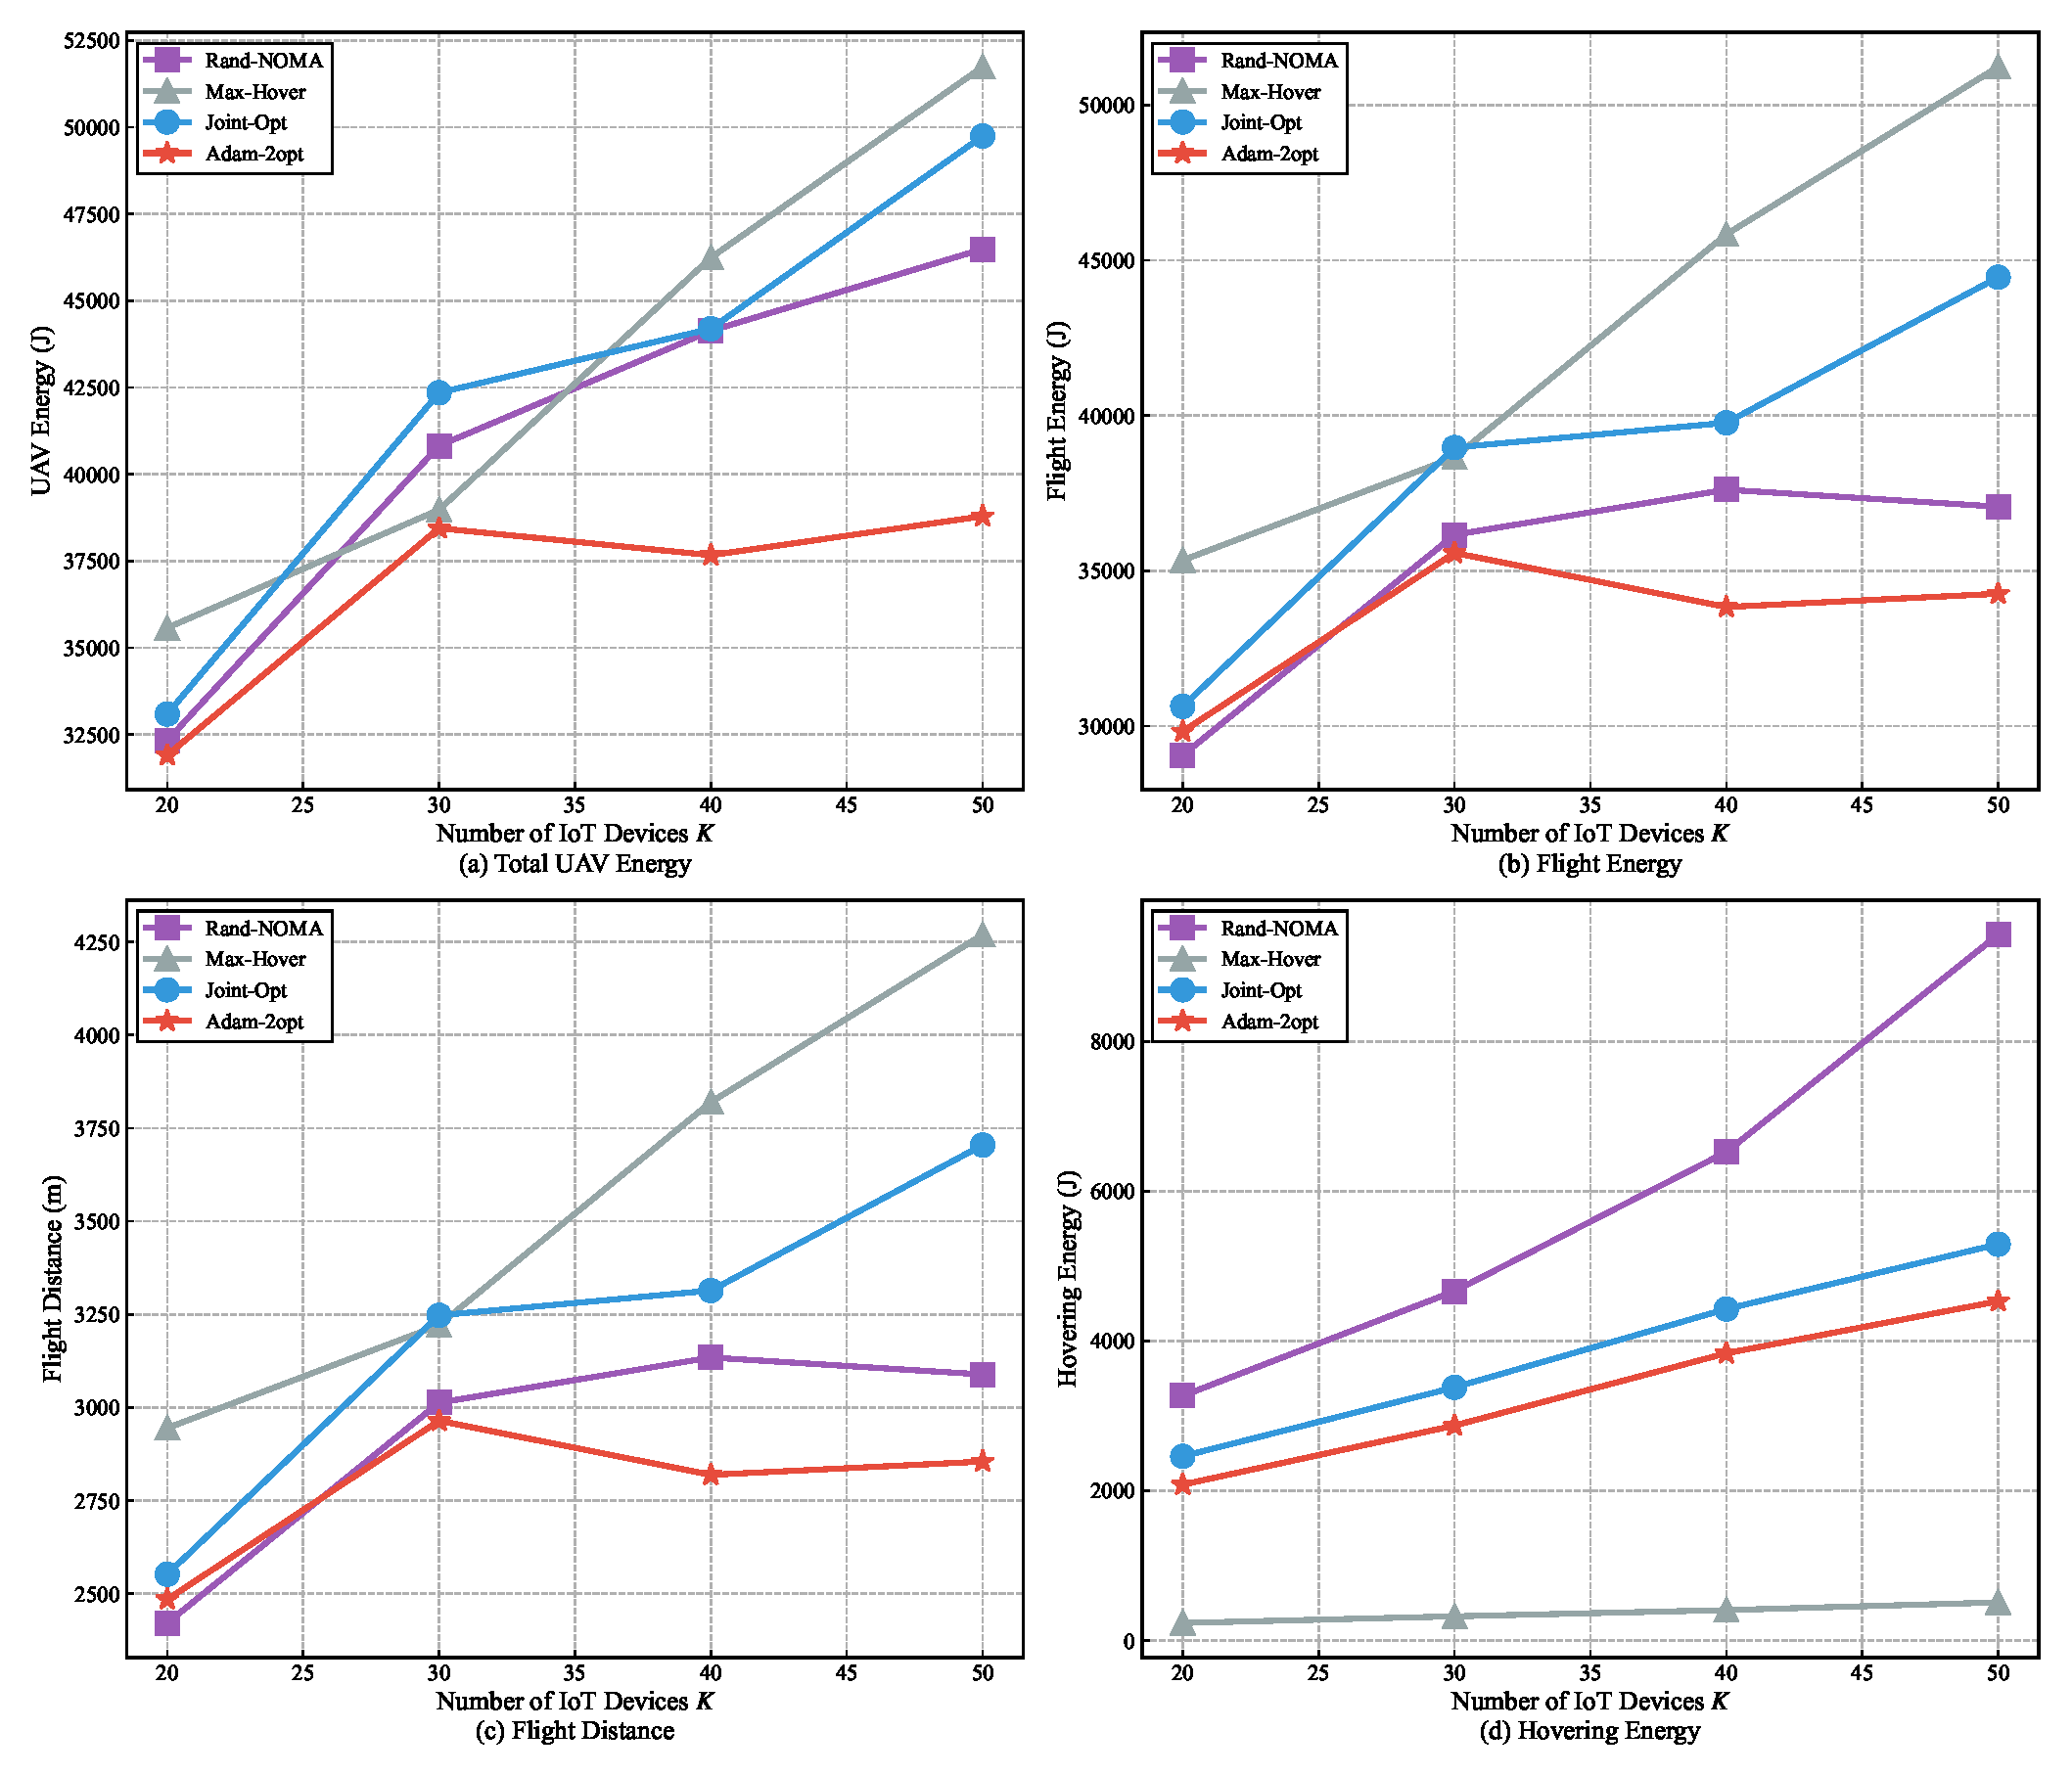
\includegraphics[width=0.95\columnwidth]{Definitions/comparison_4algorithms}
\caption{Performance comparison of different algorithms in the IoT-UAV phase.}
\label{fig:comparison_4algorithms}
\end{figure}
The first part of the evaluation focuses on the ground-to-air segment. UAVs operate within a $500\times 500~\text{m}^2$ area containing spatially distributed IoT devices, and a fixed-altitude multi-UAV configuration is adopted to reflect typical low-altitude urban deployments. Each scenario is executed under three independent random seeds, and results are averaged. To assess the effectiveness of the proposed Adam-2opt algorithm, three baseline strategies are considered: (i) \textit{Random Pairing}, which forms NOMA pairs without channel awareness; (ii) \textit{Fixed Hovering}, which prioritizes hovering duration without optimizing flight paths; and (iii) \textit{Basic Optimization}, which incorporates pairing, power allocation, and position optimization but lacks trajectory refinement.
% Figure 5
\begin{figure}[!htbp]
\centering
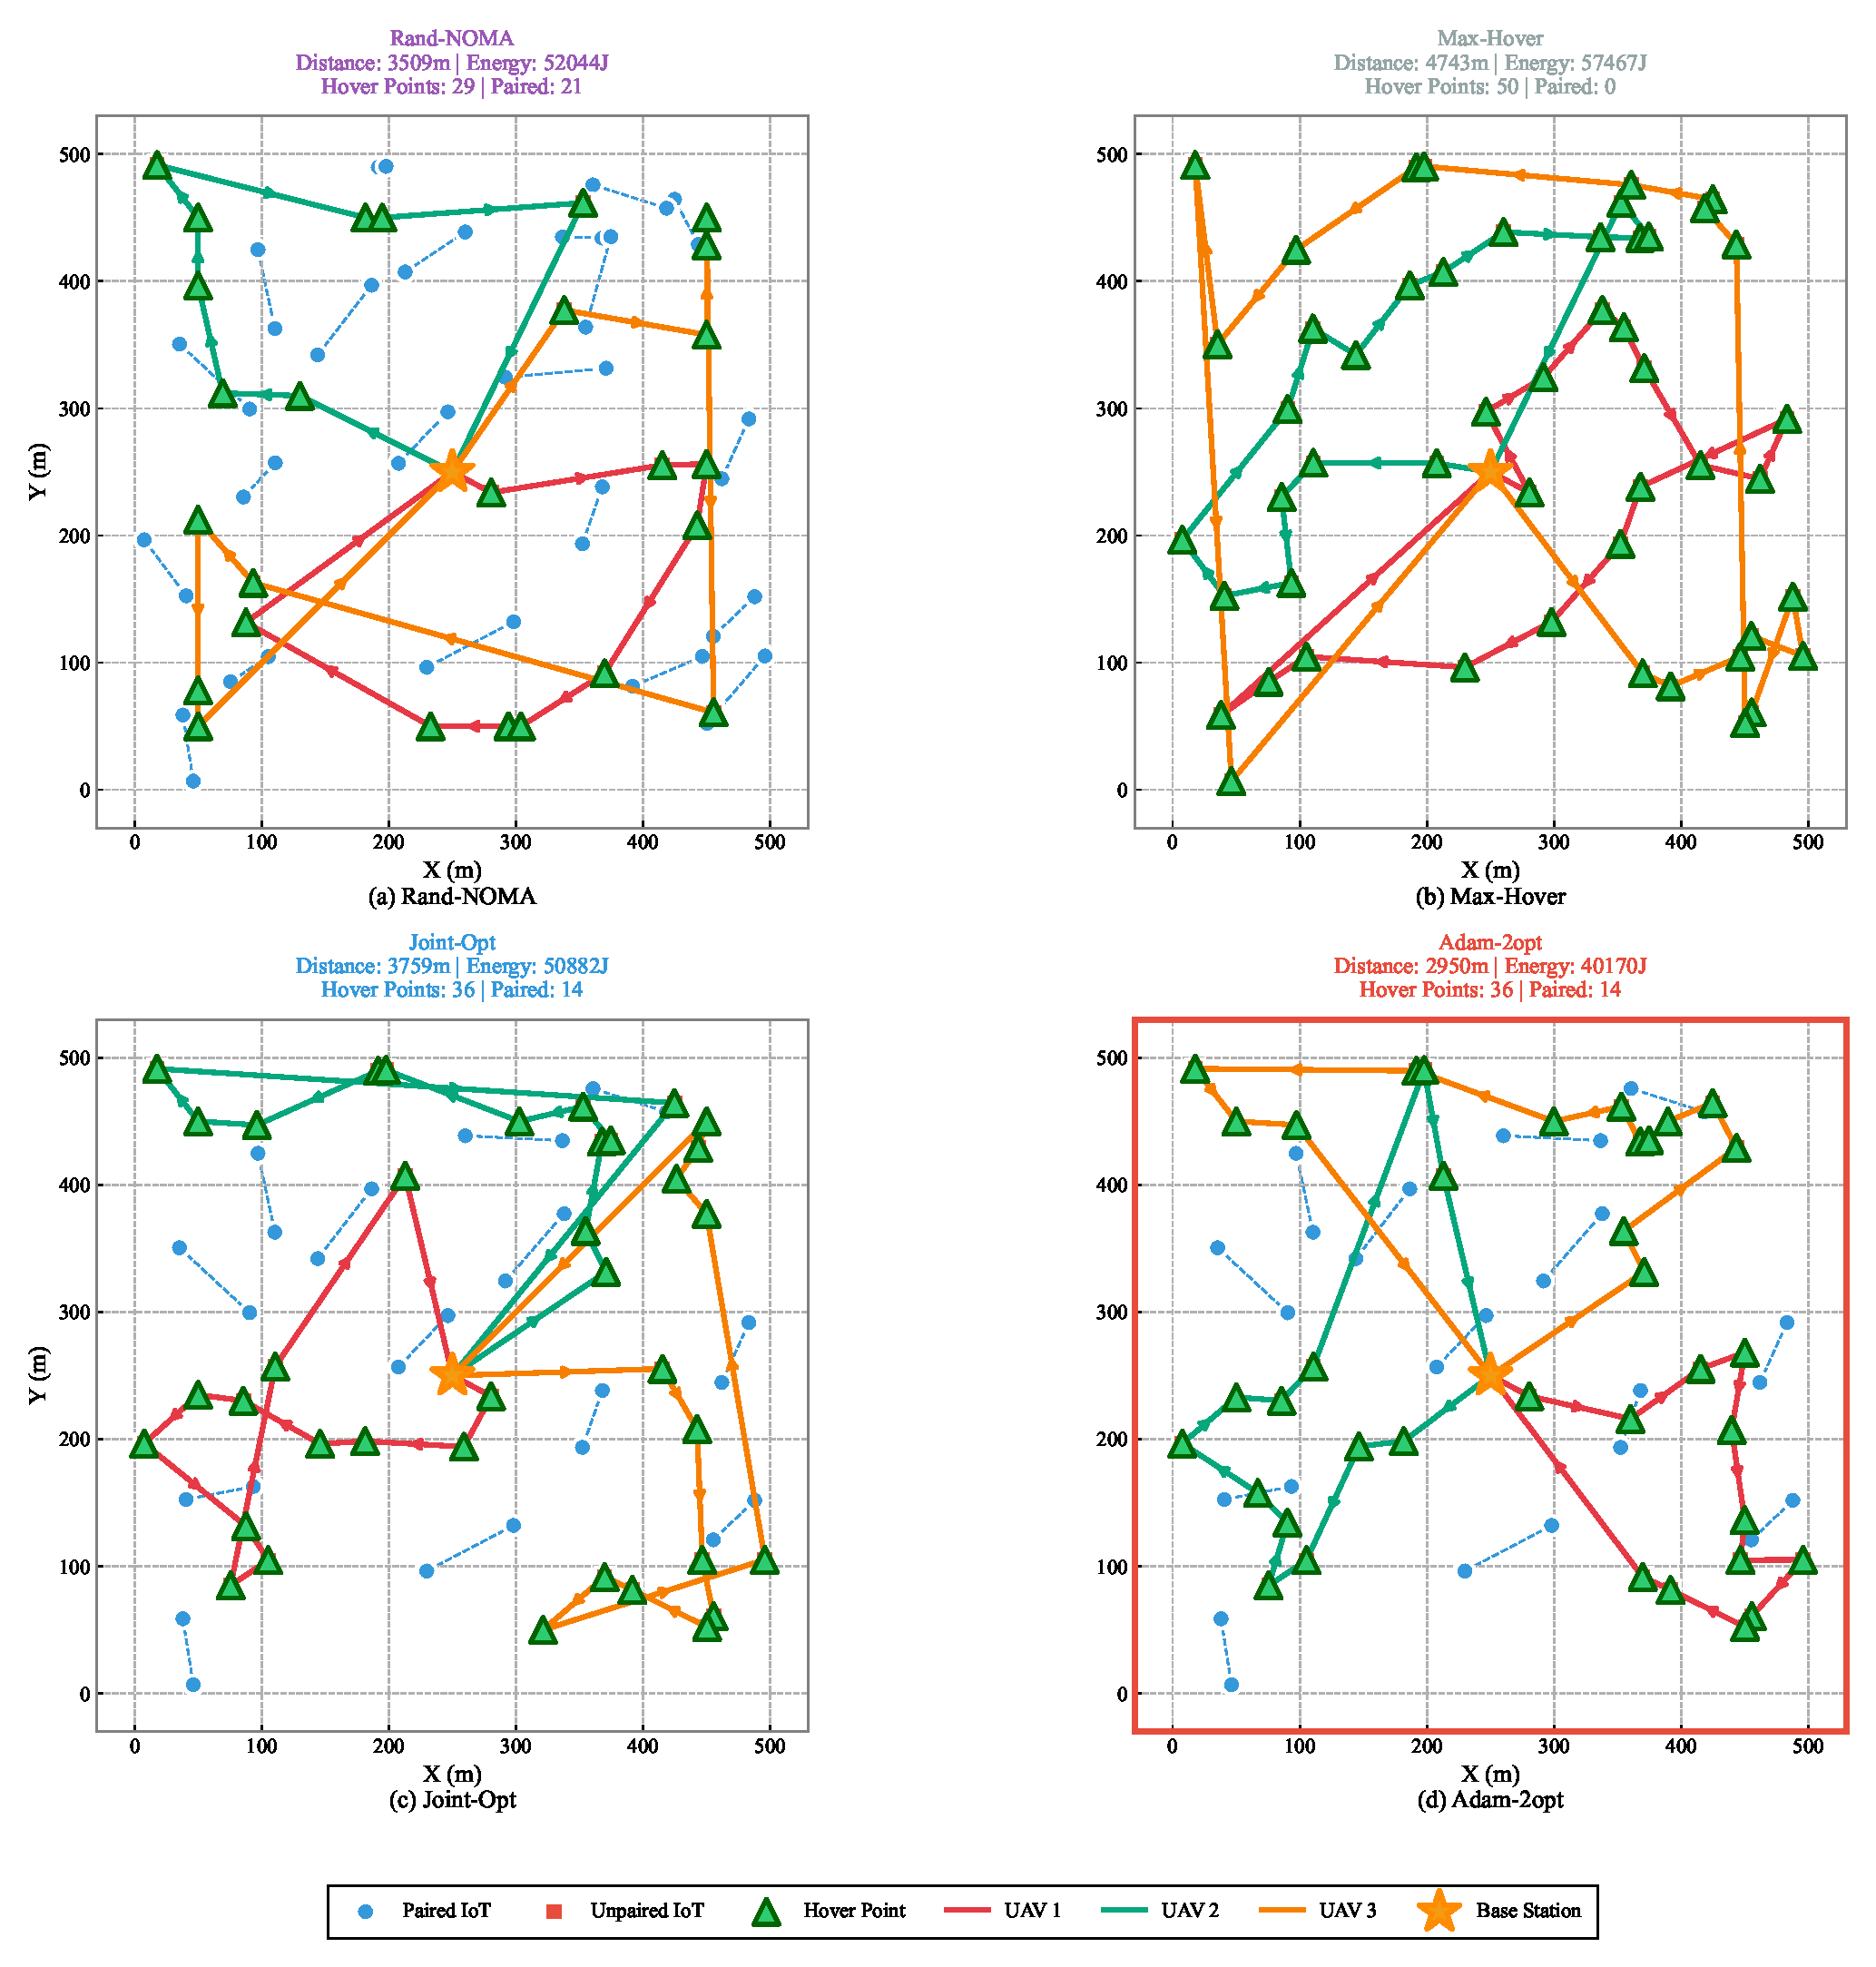
\includegraphics[width=0.95\columnwidth]{Definitions/trajectory_comparison_4algorithms}
\caption{UAV trajectory comparison between different optimization algorithms.}
\label{fig:trajectory_comparison}
\end{figure}
The second part of the evaluation examines the air-to-space offloading process. The Starlink constellation at 550~km altitude is simulated, and the number of visible satellites varies with time as the orbital geometry evolves. The UAV employs a 20~GHz carrier frequency and adheres to a minimum elevation angle constraint. A fixed interruption duration is applied to each handover event. A 10-minute evaluation window with 20-second intervals is considered, during which multiple handover opportunities arise. Two handover strategies are compared: a \textit{Greedy} scheme that always selects the satellite offering the highest instantaneous rate, and the proposed \textit{Demand-Aware} method, which performs handover only when necessary to meet the remaining offloading demand.


\subsection{Ground-to-Air Data Acquisition Performance}

The ground-to-air data acquisition stage poses a tightly coupled optimization problem involving NOMA pairing, power allocation, and UAV trajectory design. Figure~\ref{fig:comparison_4algorithms} summarizes the performance of all evaluated algorithms across four key metrics. The results consistently show that the proposed Adam-2opt method delivers the most energy-efficient operation, particularly in dense IoT deployments.

Figure~\ref{fig:comparison_4algorithms}a indicates that total UAV energy consumption increases with the number of IoT devices, yet the proposed method exhibits the slowest growth trend. While all algorithms perform similarly under low-density conditions ($K=20$), the performance gap widens significantly as the network scales. At $K=50$, Adam-2opt achieves more than 16\% energy reduction compared with Random Pairing, and over 22\% compared with Basic Optimization. This demonstrates that advanced trajectory refinement becomes increasingly valuable when device clustering and route complexity intensify. 

The primary advantage of Adam-2opt arises from its ability to simultaneously optimize hovering locations and visit sequencing. As shown in Figure~\ref{fig:comparison_4algorithms}c, the proposed design produces the shortest flight distance among all methods, with a reduction exceeding 30\% relative to Fixed Hovering at high densities. The 2-opt refinement eliminates path crossings and unnecessary detours, which directly translates into reduced flight energy, as reflected in Figure~\ref{fig:comparison_4algorithms}b. These improvements highlight the importance of trajectory-level optimization in UAV-assisted data collection.

Hovering energy behavior, depicted in Figure~\ref{fig:comparison_4algorithms}d, provides additional insight into algorithmic trade-offs. Fixed Hovering minimizes hovering time by construction but suffers from excessive flight distance, leading to the highest overall energy consumption. Random Pairing exhibits the opposite issue: arbitrary device grouping produces spatially dispersed clusters, substantially increasing hovering duration. By contrast, Adam-2opt maintains balanced performance—hovering time is reduced by nearly 50\% compared with Random Pairing—while preserving the shortest flight trajectory. This balanced design is essential for missions where both hovering and flight energy dominate total consumption.

To further illustrate spatial efficiency, Figure~\ref{fig:trajectory_comparison} visualizes representative flight paths for $K=50$. The Random Pairing trajectory (Figure~\ref{fig:trajectory_comparison}a) displays numerous crossings and backtracking segments, consistent with the disordered pairing structure. Fixed Hovering (Figure~\ref{fig:trajectory_comparison}b) generates well-spread hovering points but forces UAVs to traverse a large number of redundant waypoints. Basic Optimization (Figure~\ref{fig:trajectory_comparison}c) improves spatial locality but still retains avoidable turns and suboptimal visiting sequences. The proposed Adam-2opt trajectory (Figure~\ref{fig:trajectory_comparison}d) is notably more compact and structured, with no crossings and a clear directional flow. This confirms the complementary roles of Adam-based hovering refinement and 2-opt sequencing in producing globally efficient flight paths.

Computational cost results show that Adam-2opt requires greater planning time due to its iterative nature. However, the runtime remains on the order of one second, which is negligible for offline mission planning. The energy savings achieved—exceeding 16\% in dense deployments—far outweigh this cost, reinforcing the practicality of the approach for pre-scheduled UAV operations.

Finally, the scalability trends observed in Figure~\ref{fig:comparison_4algorithms} underline an important system-level implication. While simple heuristics suffice in small networks, their performance deteriorates rapidly with increasing density. In contrast, Adam-2opt exhibits sublinear growth in energy consumption and maintains robust performance as $K$ increases. This indicates that the proposed framework is particularly well-suited for large-scale IoT scenarios where spatial clustering and route complexity demand more sophisticated optimization.


% ==============================================================================
% 4.3 Performance of UAV-LEO Offloading Stage
% ==============================================================================
\subsection{UAV–LEO Offloading Performance}

The second stage evaluates the offloading of aggregated data from UAVs to LEO satellites, where the dominant challenge shifts from spatial optimization to managing strongly time-varying satellite visibility. Unlike the ground-to-air segment, satellite links exhibit rapid fluctuations due to orbital motion, making connection stability as critical as instantaneous link quality.
% Figure 6
\begin{figure}[!htbp]
\centering
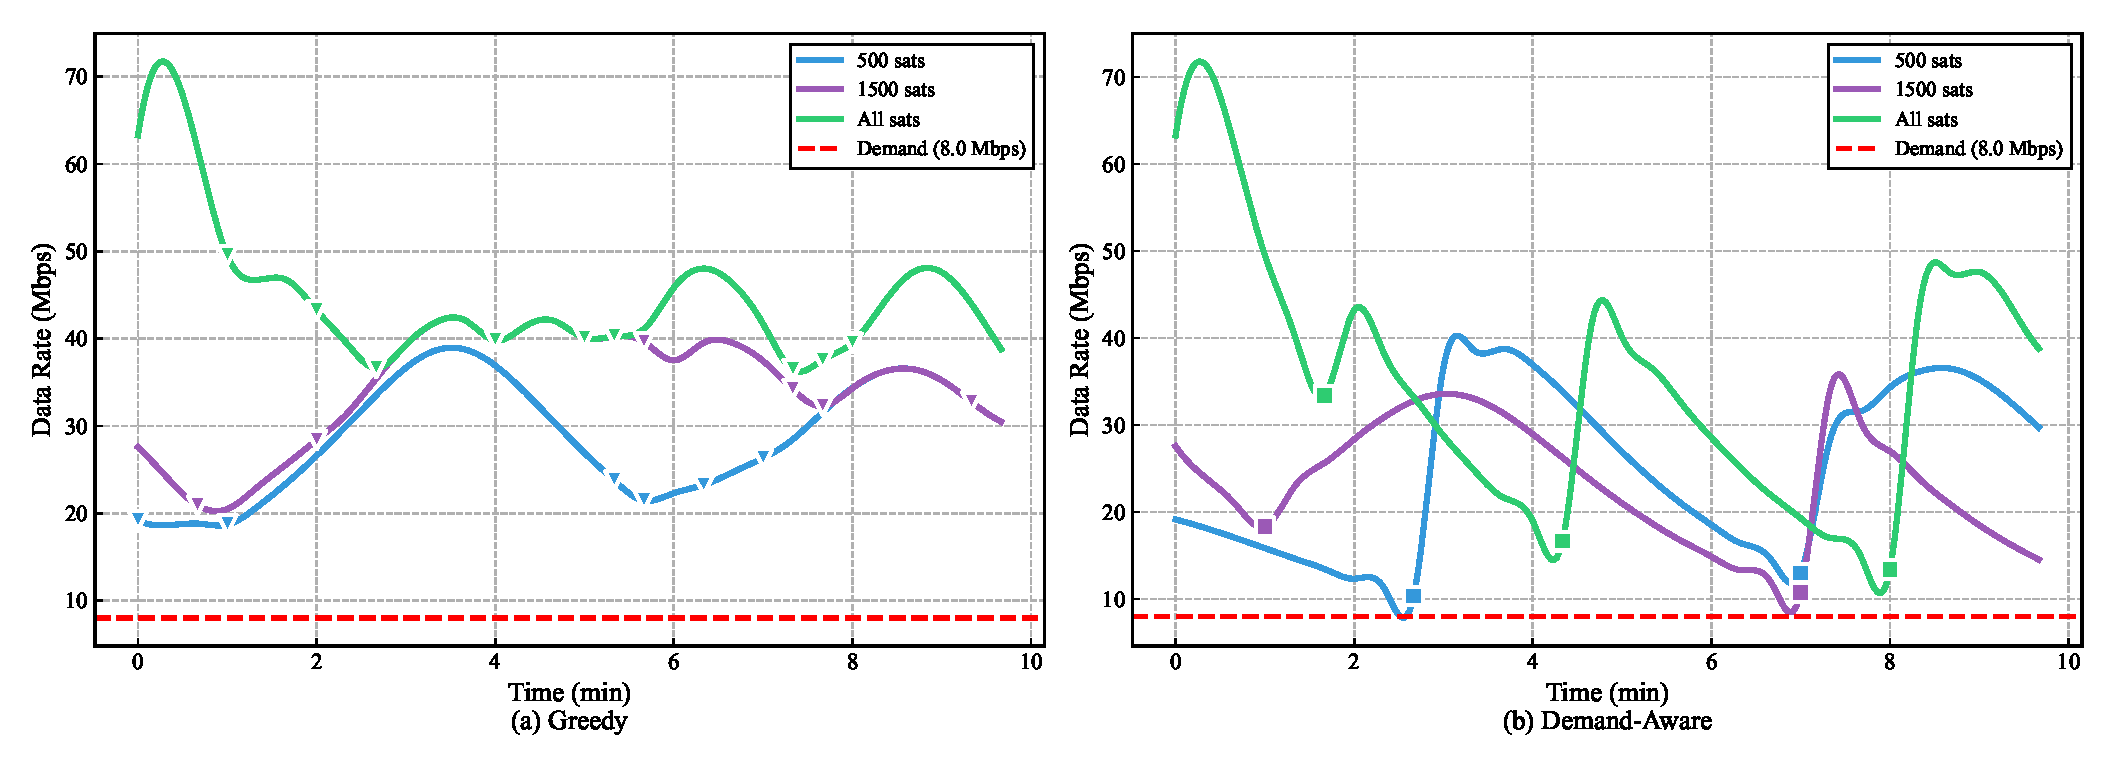
\includegraphics[width=0.95\columnwidth]{Definitions/demand_aware_number_of_satellites}
\caption{Comparison of satellite selection strategies: handover frequency versus constellation size.}
\label{fig:demand_aware_satellites}
\end{figure}
A key observation from Figure~\ref{fig:demand_aware_satellites} is the fundamental difference in handover behavior between the two evaluated strategies. The Greedy scheme continually switches to the satellite offering the highest instantaneous rate, resulting in pronounced rate volatility and frequent handover events. This behavior becomes more severe as satellite density increases, reflecting its sensitivity to instantaneous channel variations rather than long-term transmission feasibility.

In contrast, the Demand-Aware strategy produces consistently smoother rate trajectories and dramatically fewer handovers. By maintaining the current satellite connection as long as the remaining data demand can be satisfied within the predicted visibility window, the method avoids unnecessary switching and preserves link continuity. This design principle leads to a stable operating regime across all constellation densities, with only two to three handovers observed even in large constellations.
% Figure 6
\begin{figure}[!htbp]
\centering
\includegraphics[width=0.95\columnwidth]{Definitions/packet_loss_analysis}
\caption{Impact of satellite selection strategy on packet loss performance.}
\label{fig:packet_loss}
\end{figure}
Figure~\ref{fig:packet_loss}a quantitatively highlights this stability. Demand-Aware consistently reduces handover occurrences by 66--75\% relative to Greedy, and the reduction remains nearly invariant across the 500-, 1500-, and full-constellation scenarios. This invariance is particularly notable because it shows that the strategy scales gracefully with constellation size: the number of available satellites increases, but the handover count does not. Thus, Demand-Aware does not exploit satellite density to switch more frequently; instead, it leverages it to sustain longer, more reliable connections.

The practical implication of reduced handover activity is evident in the packet loss performance shown in Figure~\ref{fig:packet_loss}b. Because every handover incurs a fixed interruption period, lower switching frequency directly translates into proportionally lower loss rates. Demand-Aware maintains packet loss between 0.133\% and 0.200\%, whereas Greedy experiences losses three to four times higher. Although the absolute percentages appear small, the difference corresponds to several tens of kilobits over a typical mission—non-negligible for latency-sensitive applications such as real-time sensing or video uplink. These results demonstrate that optimizing for stability can yield a more reliable offloading process than purely maximizing instantaneous rate.

A trade-off emerges when examining average throughput. The Greedy strategy attains higher mean rates due to its aggressive switching behavior; however, this throughput advantage comes at the cost of substantial instability, packet loss, and service disruption. Demand-Aware yields 13--32\% lower average rates, but still consistently exceeds the required 8~Mbps demand by a comfortable margin. This surplus indicates that the system is operating well above its QoS threshold even without chasing maximum instantaneous rate, validating that rate maximization is not the limiting factor in this stage.

Finally, the scalability behavior across constellations provides insight into future LEO deployments. As the density of satellites increases, Greedy becomes increasingly unstable, with handover counts rising due to more frequent rate fluctuations. Demand-Aware, however, maintains nearly identical performance across all densities. This robustness arises from its demand-driven decision rule, which depends on the time required to complete the remaining offloading task rather than on short-term channel variations. Consequently, the method remains effective even as constellation sizes grow, making it well-suited for next-generation, high-density LEO systems.


\subsection{End-to-End System Analysis}

The end-to-end evaluation highlights how the two-stage optimization framework jointly enhances mission efficiency from initial IoT data acquisition to final satellite offloading. While the preceding subsections examined each stage independently, their combined behavior reveals the full benefit of coupling spatial efficiency in the ground segment with temporal stability in the space segment.

A representative mission with $K=50$ devices and 500 visible satellites illustrates this interaction. In the acquisition stage, the Adam-2opt method completes data collection with substantially reduced flight distance and energy expenditure, resulting in a shorter collection period. This improvement has direct implications for the offloading stage: by shortening the time window during which data must be transmitted, and by generating well-structured aggregated traffic, the system lowers the temporal pressure placed on the satellite link.

The offloading stage further amplifies these gains. The Demand-Aware strategy maintains stable connectivity with only two satellite handovers while sustaining data rates well above the required threshold. The reduced switching activity not only minimizes packet loss but also prevents retransmissions that would otherwise increase mission duration and UAV energy consumption. Together, the two stages form a complementary pair: the first minimizes the amount of work the second must perform under dynamic link conditions, while the second ensures reliable and efficient transfer of the data produced by the first.

Table~\ref{tab:end_to_end_comparison} summarizes the resulting system-level improvements. The proposed framework achieves simultaneous reductions in UAV energy consumption, flight distance, collection time, handover count, and packet loss. Although the average offloading rate is modestly lower than that of the Greedy strategy, it remains well above the demand threshold, confirming that meeting quality-of-service requirements does not require maximizing instantaneous throughput. Instead, the results show that stability-driven offloading yields superior system performance across all metrics of operational relevance.

The scalability characteristics further emphasize the robustness of the design. As IoT device density increases, the benefits of spatial optimization become more pronounced, with energy savings rising from marginal levels at low density to double-digit improvements at higher density. Conversely, the performance of the offloading stage remains largely unaffected by ground-segment scaling, consistently limiting handovers to two or three events regardless of IoT density. This decoupling is desirable: Algorithm~1 efficiently adapts to spatial complexity on the ground, while Algorithm~2 maintains stable performance in the space segment independent of the ground network.

Satellite density variation produces a similar conclusion. The Greedy strategy becomes increasingly unstable as constellation density grows, whereas the Demand-Aware approach exhibits nearly constant switching behavior. This insensitivity to satellite availability reflects a fundamental advantage of demand-based switching: decisions are driven by transmission requirements rather than by short-term channel fluctuations. As next-generation LEO constellations continue to expand, such robustness will be essential for ensuring reliable large-scale UAV–satellite integration.

Overall, the end-to-end evaluations demonstrate that optimizing spatial and temporal dimensions jointly, rather than individually, yields substantial system-level gains. By aligning the objectives of ground-level trajectory design with those of satellite-level handover management, the proposed framework supports efficient, reliable, and scalable operation across heterogeneous segments of the SAGIN architecture.

%%%%%%%%%%%%%%%%%%%%%%%%%%%%%%%%%%%%%%%%%%
\section{Discussion}

The simulation results provide several overarching insights into the design of integrated UAV-assisted IoT collection and LEO satellite offloading systems. Beyond validating the performance gains of the proposed algorithms, the findings highlight structural principles that can inform future SAGIN architectures.

A central observation is that effective UAV trajectory planning requires joint reasoning over multiple coupled spatial objectives. Approaches that optimize hovering locations or hovering duration in isolation fail to capture the interdependence between waypoint placement and path structure. The Adam-2opt strategy illustrates that combining continuous refinement of hovering positions with discrete trajectory optimization yields substantially better performance than either technique alone. This supports a broader design principle: in spatially distributed IoT systems, hybrid optimization methods that exploit both geometric structure and combinatorial refinement can unlock performance regimes unattainable through single-method strategies.

In the LEO offloading stage, the Demand-Aware handover mechanism represents a shift from instantaneous-metric optimization toward stability-oriented decision making. Traditional handover strategies prioritize maximizing instantaneous throughput or SNR, but the experiments show that such myopic optimization leads to excessive switching and degraded reliability. By contrast, Demand-Aware operates under a sufficiency-based philosophy: as long as the current link can support the remaining offloading requirement, switching is unnecessary. This insight underscores the importance of aligning optimization objectives with mission-level guarantees rather than maximizing transient performance metrics. In dynamic satellite environments, optimizing \textit{link continuity} can be more valuable than optimizing \textit{peak throughput}.

The interaction between the two stages reveals another key design implication: spatial and temporal optimizations should be complementary rather than independent. Algorithm~1 reduces the volume and timing variability of data entering the satellite offloading stage, while Algorithm~2 provides a stable communication channel whose reliability minimizes retransmissions and wasted energy. Their objectives reinforce rather than compete with each other, demonstrating that decomposing a complex end-to-end mission into coordinated subproblems can yield near-optimal global behavior when the interfaces between stages are properly aligned.

These findings also shed light on the limitations of a hypothetical fully integrated optimization framework. Although jointly optimizing UAV trajectories and satellite handovers may appear ideal, the drastically different temporal scales of the two processes make such integration impractical. UAV trajectory planning evolves on minute-level horizons with predictable spatial structure, while satellite handovers occur on the order of seconds and depend on rapidly changing orbital geometry. Treating both processes within a single optimization loop would either render trajectory planning computationally intractable or slow down handover decisions beyond usable limits. The proposed two-stage separation thus reflects not only a computational convenience but a necessary architectural decision that respects the heterogeneous dynamics of SAGIN systems.

The computational cost associated with the Adam-2opt method further highlights an important trade-off in system design. Although the algorithm incurs modest additional planning time compared to simplified baselines, this overhead remains negligible in the context of offline mission scheduling. The significant energy savings achieved by the method—critical for extending UAV operational range—justify the additional computational effort. For real-time adaptation scenarios, lighter-weight approximations could be employed, but the results suggest that when planning time is not a bottleneck, more expressive optimization procedures yield substantial benefits.

Scalability trends observed in the experiments reinforce the value of sophisticated optimization in large-scale SAGIN deployments. As IoT device density increases, baseline methods degrade rapidly, whereas the proposed trajectory optimizer maintains controlled energy growth. Likewise, the Demand-Aware handover strategy exhibits remarkably stable performance across a wide range of satellite densities, indicating that its decision rule naturally generalizes to future high-density constellations. These scaling behaviors demonstrate that robustness to network expansion should be a first-class objective in SAGIN system design, especially given the accelerating growth of IoT deployments and commercial LEO constellations.

Finally, several practical considerations emerge for real-world adoption. In UAV trajectory planning, uncertainties in channel state information and device mobility may require incorporating robust or prediction-based extensions. In the satellite segment, adaptive demand thresholds or coordinated multi-UAV handover control could further enhance stability. These enhancements are compatible with the modularity of the proposed framework, which allows each stage to evolve independently while maintaining system-level coherence.

Overall, the discussion highlights that efficient SAGIN operation depends not solely on isolated algorithmic performance but on aligning optimization principles across spatial and temporal domains. By designing stage-specific strategies that respect the intrinsic dynamics of their respective environments, the proposed framework demonstrates how modular yet complementary optimization can yield reliable, scalable, and energy-efficient end-to-end mission performance.

%%%%%%%%%%%%%%%%%%%%%%%%%%%%%%%%%%%%%%%%%%
\section{Conclusions}

This work developed a two-stage optimization framework for UAV-assisted IoT data collection and LEO satellite offloading in SAGIN environments. The proposed approach integrates spatial optimization for UAV trajectory planning with temporal optimization for satellite handover management, addressing the fundamentally different dynamics of the ground-to-air and air-to-space segments. Through extensive simulations, the framework demonstrated substantial gains in energy efficiency, trajectory compactness, connectivity stability, and end-to-end reliability compared with baseline strategies.

A key contribution of this study is the identification of complementary optimization principles across heterogeneous network layers. The Adam-2opt method leverages continuous and discrete optimization to construct energy-efficient collection trajectories, while the Demand-Aware handover strategy adopts a sufficiency-based decision rule that prioritizes link continuity over instantaneous throughput. Their combined operation illustrates how aligning spatial and temporal objectives can produce superior end-to-end performance without requiring a fully integrated or computationally prohibitive joint optimization.

The observed scalability properties further highlight the framework's suitability for emerging large-scale SAGIN deployments. The UAV trajectory optimizer becomes increasingly advantageous as IoT densities grow, while the handover strategy remains robust to expanding LEO constellation sizes. These characteristics position the framework as a practical and future-proof solution for next-generation aerial–satellite–terrestrial IoT systems.

Future extensions of this work may incorporate uncertainty-aware trajectory planning, adaptive demand thresholds for dynamic offloading, and cooperative multi-UAV handover coordination. Despite these opportunities, the proposed methods already achieve strong performance with modest computational overhead, making them readily applicable to real-world mission planning and execution.

Overall, this study demonstrates that modular yet complementary optimization across network segments can substantially enhance the efficiency and reliability of SAGIN architectures, offering a promising direction for the design of integrated aerial–satellite IoT systems.

%%%%%%%%%%%%%%%%%%%%%%%%%%%%%%%%%%%%%%%%%%
%\isPreprints{} % If the paper is ``preprints'', please uncomment this parenthesis.
%\printendnotes[custom] % Un-comment to print a list of endnotes

\reftitle{References}

% Please provide the correct journal abbreviation (e.g. according to the “List of Title Word Abbreviations” http://www.issn.org/services/online-services/access-to-the-ltwa/).
% Citations and References in Supplementary files are permitted provided that they also appear in the reference list here. 

%=====================================
% References, variant A: external bibliography
%=====================================
% \bibliography{your_external_BibTeX_file}

%=====================================
% References, variant B: internal bibliography
%=====================================

% ACS format
\begin{thebibliography}{999}
% Reference 1
\bibitem{jia2020leo}
Jia, Z.; Sheng, M.; Li, J.; Niyato, D.; Han, Z.
LEO-satellite-assisted UAV: Joint trajectory and data collection for Internet of Remote Things in 6G aerial access networks.
{\em IEEE Internet Things J.} {\bf 2020}, {\em 8}, 9814--9826.

% Reference 2
\bibitem{xiao2024space}
Xiao, Y.; Ye, Z.; Wu, M.; Li, H.; Xiao, M.; Alouini, M.-S.; Al-Hourani, A.; Cioni, S.
Space-air-ground integrated wireless networks for 6G: Basics, key technologies and future trends.
{\em IEEE J. Sel. Areas Commun.} {\bf 2024}.

% Reference 3
\bibitem{duan2022distributed}
Duan, S.; Wang, D.; Ren, J.; Lyu, F.; Zhang, Y.; Wu, H.; Shen, X.
Distributed artificial intelligence empowered by end-edge-cloud computing: A survey.
{\em IEEE Commun. Surv. Tutor.} {\bf 2022}, {\em 25}, 591--624.

% Reference 4
\bibitem{wei2024energy}
Wei, Q.; Chen, Y.; Jia, Z.; Bai, W.; Pei, T.; Wu, Q.
Energy-efficient caching and user selection for resource-limited SAGINs in emergency communications.
{\em IEEE Trans. Commun.} {\bf 2024}.

% Reference 5
\bibitem{pan2022latency}
Pan, G.; Ye, J.; An, J.; Alouini, M.-S.
Latency versus reliability in LEO mega-constellations: Terrestrial, aerial, or space relay?
{\em IEEE Trans. Mob. Comput.} {\bf 2022}, {\em 22}, 5330--5345.

% Reference 6
\bibitem{jia2025distributionally}
Jia, Z.; Cui, C.; Dong, C.; Wu, Q.; Ling, Z.; Niyato, D.; Han, Z.
Distributionally robust optimization for aerial multi-access edge computing via cooperation of UAVs and HAPs.
{\em IEEE Trans. Mob. Comput.} {\bf 2025}.

% Reference 7
\bibitem{mao2020joint}
Mao, S.; He, S.; Wu, J.
Joint UAV position optimization and resource scheduling in space-air-ground integrated networks with mixed cloud-edge computing.
{\em IEEE Syst. J.} {\bf 2020}, {\em 15}, 3992--4002.

% Reference 8
\bibitem{zhao2021multi}
Zhao, C.; Liu, J.; Sheng, M.; Teng, W.; Zheng, Y.; Li, J.
Multi-UAV trajectory planning for energy-efficient content coverage: A decentralized learning-based approach.
{\em IEEE J. Sel. Areas Commun.} {\bf 2021}, {\em 39}, 3193--3207.
% Reference 9
\bibitem{mozaffari2019tutorial}
Mozaffari, M.; Saad, W.; Bennis, M.; Nam, Y.-H.; Debbah, M.
A tutorial on UAVs for wireless networks: Applications, challenges, and open problems.
{\em IEEE Commun. Surv. Tutor.} {\bf 2019}, {\em 21}, 2334--2360.
% Reference 10
\bibitem{tao2015survey}
Tao, Y.; Liu, L.; Liu, S.; Zhang, Z.
A survey: Several technologies of non-orthogonal transmission for 5G.
{\em China Commun.} {\bf 2015}, {\em 12}, 1--15.
% Reference 11
\bibitem{fang2022noma}
Fang, X.; Feng, W.; Wang, Y.; Chen, Y.; Ge, N.; Ding, Z.; Zhu, H.
NOMA-based hybrid satellite-UAV-terrestrial networks for 6G maritime coverage.
{\em IEEE Trans. Wireless Commun.} {\bf 2022}, {\em 22}, 138--152.
% Reference 12
\bibitem{jia2025service}
Jia, Z.; Cao, Y.; He, L.; Wu, Q.; Zhu, Q.; Niyato, D.; Han, Z.
Service function chain dynamic scheduling in space-air-ground integrated networks.
{\em IEEE Trans. Veh. Technol.} {\bf 2025}.
% Reference 13
\bibitem{huang2024joint}
Huang, C.; Chen, G.; Xiao, P.; Xiao, Y.; Han, Z.; Chambers, J. A.
Joint offloading and resource allocation for hybrid cloud and edge computing in SAGINs: A decision assisted hybrid action space deep reinforcement learning approach.
{\em IEEE J. Sel. Areas Commun.} {\bf 2024}, {\em 42}, 1029--1043.
% Reference 14
\bibitem{jia2024dynamic}
Jia, H.; Wang, Y.; Wu, W.
Dynamic resource allocation for remote IoT data collection in SAGIN.
{\em IEEE Internet Things J.} {\bf 2024}, {\em 11}, 20575--20589.
% Reference 15
\bibitem{seyedi2012trace}
Seyedi, Y.; Rahimi, F.
A trace-time framework for prediction of elevation angle over land mobile LEO satellites networks.
{\em Wirel. Pers. Commun.} {\bf 2012}, {\em 62}, 793--804.
% Reference 16
\bibitem{d2020learning}
d O Costa, P. R.; Rhuggenaath, J.; Zhang, Y.; Akcay, A.
Learning 2-opt heuristics for the traveling salesman problem via deep reinforcement learning.
{\em Asian Conf. Mach. Learn.} {\bf 2020}, 465--480.

\end{thebibliography}

% If authors have biography, please use the format below
%\section*{Short Biography of Authors}
%\bio
%{\raisebox{-0.35cm}{\includegraphics[width=3.5cm,height=5.3cm,clip,keepaspectratio]{Definitions/author1.pdf}}}
%{\textbf{Firstname Lastname} Biography of first author}
%
%\bio
%{\raisebox{-0.35cm}{\includegraphics[width=3.5cm,height=5.3cm,clip,keepaspectratio]{Definitions/author2.jpg}}}
%{\textbf{Firstname Lastname} Biography of second author}

% For the MDPI journals use author-date citation, please follow the formatting guidelines on http://www.mdpi.com/authors/references
% To cite two works by the same author: \citeauthor{ref-journal-1a} (\citeyear{ref-journal-1a}, \citeyear{ref-journal-1b}). This produces: Whittaker (1967, 1975)
% To cite two works by the same author with specific pages: \citeauthor{ref-journal-3a} (\citeyear{ref-journal-3a}, p. 328; \citeyear{ref-journal-3b}, p.475). This produces: Wong (1999, p. 328; 2000, p. 475)

%%%%%%%%%%%%%%%%%%%%%%%%%%%%%%%%%%%%%%%%%%
%% for journal Sci
%\reviewreports{\\
%Reviewer 1 comments and authors’ response\\
%Reviewer 2 comments and authors’ response\\
%Reviewer 3 comments and authors’ response
%}
%%%%%%%%%%%%%%%%%%%%%%%%%%%%%%%%%%%%%%%%%%
\begin{comment}
\PublishersNote{}
\end{comment}
%\isPreprints{} % If the paper is ``preprints'', please uncomment this parenthesis.

\end{document}


